\documentclass[11pt]{article}
\usepackage[T1]{fontenc}
\usepackage{lmodern,microtype}
\usepackage[margin=1in]{geometry}
\usepackage{amsmath,amssymb,amsthm,mathtools}
\usepackage{enumitem,graphicx,tikz,xcolor,array,booktabs,tabularx}
\usetikzlibrary{arrows.meta,calc,positioning,patterns}
\usepackage[colorlinks=true,linkcolor=teal!55!black,citecolor=teal!55!black,urlcolor=teal!55!black]{hyperref}
\hypersetup{pdftitle={The critical correlation exponent of the planar XY model},pdfauthor={OpenAI}}
\setlength{\emergencystretch}{1em}
\setlist{itemsep=3pt,topsep=5pt}
\numberwithin{equation}{section}
\newtheorem{theorem}{Theorem}[section]
\newtheorem{lemma}[theorem]{Lemma}
\newtheorem{proposition}[theorem]{Proposition}
\newtheorem{corollary}[theorem]{Corollary}
\theoremstyle{definition}
\newtheorem{definition}[theorem]{Definition}
\theoremstyle{remark}
\newtheorem{remark}[theorem]{Remark}
\newcommand{\R}{\mathbb R}
\newcommand{\Z}{\mathbb Z}
\newcommand{\N}{\mathbb N}
\newcommand{\T}{\mathbb T}
\newcommand{\E}{\mathbb E}
\newcommand{\Prob}{\mathbb P}
\DeclareMathOperator{\Var}{Var}
\DeclareMathOperator{\Cov}{Cov}
\DeclareMathOperator{\supp}{supp}
\DeclareMathOperator{\dist}{dist}
\DeclareMathOperator{\diam}{diam}
\DeclareMathOperator{\tr}{tr}
\DeclareMathOperator{\Id}{Id}
\newcommand{\eps}{\varepsilon}
\newcommand{\ip}[2]{\langle #1,#2\rangle}
\newcommand{\norm}[1]{\lVert #1\rVert}
\newcommand{\abs}[1]{\lvert #1\rvert}
\newcommand{\dd}{\,\mathrm d}
\DeclareRobustCommand{\Bcite}[1]{%
  \ifcsname BKTref@#1\endcsname
    \cite[\csname BKTref@#1\endcsname]{BKT}%
  \else
    \PackageError{source-refs}{Unknown companion reference #1}{Use a verified numbered companion reference.}%
  \fi}
\expandafter\def\csname BKTref@an:band-density\endcsname{Lemma~3.1}
\expandafter\def\csname BKTref@an:forms\endcsname{Lemma~3.12}
\expandafter\def\csname BKTref@an:gaussian-localization\endcsname{Proposition~3.14}
\expandafter\def\csname BKTref@an:geometry\endcsname{Definition~3.11}
\expandafter\def\csname BKTref@an:mixed-scaling\endcsname{Proposition~3.13}
\expandafter\def\csname BKTref@an:path-poincare\endcsname{Lemma~3.2}
\expandafter\def\csname BKTref@an:reach\endcsname{Proposition~3.7}
\expandafter\def\csname BKTref@an:relative-pin-bound\endcsname{Equation~(3.47)}
\expandafter\def\csname BKTref@an:sign-disintegration\endcsname{Equation~(3.8)}
\expandafter\def\csname BKTref@an:tilt\endcsname{Lemma~3.6}
\expandafter\def\csname BKTref@en:bad-box\endcsname{Equation~(9.24)}
\expandafter\def\csname BKTref@en:energy-contraction\endcsname{Equation~(9.15)}
\expandafter\def\csname BKTref@en:entry\endcsname{Theorem~9.1}
\expandafter\def\csname BKTref@en:entry-covariance\endcsname{Equation~(9.11)}
\expandafter\def\csname BKTref@en:exact-density\endcsname{Equation~(9.2)}
\expandafter\def\csname BKTref@en:good-box\endcsname{Lemma~9.4}
\expandafter\def\csname BKTref@en:imaginary-wall\endcsname{Equation~(9.31)}
\expandafter\def\csname BKTref@en:link-matrix\endcsname{Equation~(9.9)}
\expandafter\def\csname BKTref@en:links\endcsname{Equation~(9.10)}
\expandafter\def\csname BKTref@en:norm\endcsname{Equation~(9.3)}
\expandafter\def\csname BKTref@en:normalization\endcsname{Lemma~9.3}
\expandafter\def\csname BKTref@en:patches\endcsname{Section~9.2}
\expandafter\def\csname BKTref@en:placement\endcsname{Equation~(9.34)}
\expandafter\def\csname BKTref@en:prediction\endcsname{Equation~(9.23)}
\expandafter\def\csname BKTref@en:regulator\endcsname{Lemma~9.2}
\expandafter\def\csname BKTref@en:seam-cost\endcsname{Equation~(9.21)}
\expandafter\def\csname BKTref@en:shifted-box\endcsname{Equation~(9.20)}
\expandafter\def\csname BKTref@en:theta-parity\endcsname{Equation~(9.29)}
\expandafter\def\csname BKTref@en:variational\endcsname{Equation~(9.13)}
\expandafter\def\csname BKTref@ep:gapped-B\endcsname{Equation~(10.10)}
\expandafter\def\csname BKTref@ep:gapped-u\endcsname{Equation~(10.11)}
\expandafter\def\csname BKTref@ep:gaussian-curves\endcsname{Lemma~10.3}
\expandafter\def\csname BKTref@ep:gradient-diagnostic\endcsname{Equation~(10.3)}
\expandafter\def\csname BKTref@rg:geometry\endcsname{Lemma~4.3}
\expandafter\def\csname BKTref@rg:regulator\endcsname{Lemma~4.4}
\expandafter\def\csname BKTref@st:coefficient-transfer\endcsname{Equation~(2.6)}
\expandafter\def\csname BKTref@st:critical-face-ratio\endcsname{Lemma~2.4}
\expandafter\def\csname BKTref@st:face-energy-bound\endcsname{Equation~(2.23)}
\expandafter\def\csname BKTref@st:finite-gaussian\endcsname{Lemma~2.1}
\expandafter\def\csname BKTref@st:fractional-mean\endcsname{Theorem~2.3}
\expandafter\def\csname BKTref@st:free-rectangle-limit\endcsname{Theorem~2.2}
\expandafter\def\csname BKTref@st:radial-cost\endcsname{Equation~(2.25)}
\expandafter\def\csname BKTref@wh:map\endcsname{Proposition~8.3}

\title{The critical correlation exponent\\of the planar XY model}
\author{OpenAI}
\date{September 24, 2026}
\begin{document}
\maketitle
\begin{abstract}
For the ordinary nearest-neighbor XY model on the square lattice,
we prove the Berezinskii--Kosterlitz--Thouless prediction that the
critical spin-correlation exponent is \(1/4\). More precisely, at
the mass-defined critical inverse temperature, the infinite-volume
correlation is \(n^{-1/4+o(1)}\). The infinite-volume limit through
free square boxes is taken before the separation limit.
\end{abstract}

\section{Introduction}
The two-dimensional XY model has an algebraic phase even though
its spins have no preferred direction.  The
Berezinskii--Kosterlitz--Thouless theory predicts that the
correlation exponent at the boundary of that phase is exactly
\(1/4\) \cite{Berezinskii,BKT1973,Kosterlitz1974}.  This paper
proves that prediction for the nearest-neighbor cosine interaction
on the square lattice, at the threshold defined by vanishing
horizontal mass.  The conclusion concerns free-box
infinite-volume correlations at all integer separations.

Several earlier results establish the surrounding phase picture.
McBryan and Spencer proved power-law upper bounds for planar
spin correlations \cite{McBryanSpencer1977}. Fr\"ohlich and
Spencer proved the existence of the low-temperature algebraic
phase by a Coulomb-gas analysis \cite{FS}. Van Engelenburg and
Lis obtained the exponential-versus-polynomial dichotomy, including
a polynomial lower bound at the threshold, by directed currents
and dual heights \cite{vEL}.  Their critical lower bound is the
external endpoint input used here; its exponent is not sharp.

The dual-height approach also has a substantial independent
history. Aizenman, Harel, Peled, and Shapiro developed
integer-restricted Gaussian and annealed Gaussian methods for
depinning and BKT phases, including a Gaussian-mixture
representation of Bessel weights \cite{AHPS2022}.
Lammers identified the exact relation between XY mass and its
dual height mass \cite{LammersBijecting2023}, and proved a
qualitative localization dichotomy with a positive universal
height-variance gap \cite{LammersDichotomy2026}.  The broader
duality identities of van Engelenburg and Lis
\cite{vanEngelenburgLisDuality2025} and the surface-tension
derivative formula of Durand and Lammers \cite{DurandLammers2026}
further connect spin decay and height fluctuations. These results
do not identify the endpoint coefficient or its magnetic
correlation exponent. Those two identifications are the tasks
addressed below.

Our companion article \cite{BKT} supplies the finite Gaussian
comparisons, annular geometry and Gaussian estimates, and local
analytic maps used in the proof. Its discrete-height theorems
concern quadratic weights, and its spin theorem concerns
sufficiently low fixed temperatures. We therefore prove the
model-specific transfers to the Bessel interaction in this paper.
Every companion citation gives a numbered statement or equation.
Section~\ref{sec:interfaces}
specifies the hypotheses at these interfaces.

Three extensions are particularly important. First, a subdivision
by lattice Gaussian chains transfers finite comparisons to Bessel
weights, but not their bare Gaussian variance bound. Unit-edge
flow costs and arbitrarily high polynomial moments replace that
bound, including after cable exploration and for very small pin
probabilities. Second, convergence of ordinary height observations
does not determine a winding-sector partition ratio. A finite
isolation expansion on geometric annuli supplies that comparison,
with only a small error per annular scale. Third, an additional
positive form on \emph{averages}, rather than on microscopic
heights, supplies the large-field reserve needed for an open
Gaussian regime. This form is removed by a variance comparison
before drawing a conclusion about the original model.

\subsection{Model and statement}
For an integer \(L\ge1\), put
\[
 \Lambda_L=[-L,L]^2\cap\Z^2,
 \qquad
 E_L=\{\{x,y\}\subset\Lambda_L:|x-y|=1\}.
\]
Every edge occurs once. At inverse temperature \(b>0\), the angles
\(\theta_x\in\R/(2\pi\Z)\) have law
\begin{equation}\label{eq:xy-law}
 \dd\mu_{L,b}(\theta)
 =Z_{L,b}^{-1}
   \exp\!\left\{b\sum_{\{x,y\}\in E_L}
                 \cos(\theta_x-\theta_y)\right\}
   \prod_{x\in\Lambda_L}\frac{\dd\theta_x}{2\pi}.
\end{equation}
There are no exterior edges, fixed spins, fields, or boundary
identifications. With \(e_1=(1,0)\), set
\begin{equation}\label{eq:correlation}
 C_b(n)=\lim_{\substack{L\to\infty\\L\ge n}}
  \E_{\mu_{L,b}}\cos(\theta_0-\theta_{ne_1}),\qquad
 m(b)=\lim_{n\to\infty}-\frac1n\log C_b(n),
\end{equation}
and
\begin{equation}\label{eq:critical-definition}
 b_c=\inf\{b>0:m(b)=0\}.
\end{equation}
The correlation limit exists by ferromagnetic coupling
monotonicity \cite{Ginibre1970}. The multiplicative correlation
inequality \cite[arXiv version~2, Lemma~19]{vEL}, after free exhaustion and
translation invariance, gives
\(C_b(n+m)\ge C_b(n)C_b(m)\). Fekete's lemma therefore gives
the mass limit. The dichotomy in \cite[Theorem~1]{vEL} implies
\(0<b_c<\infty\) and includes \(b_c\) in the massless regime.
The parameter \(b\) is exactly
the \(\beta\) of the usual cosine convention. Throughout the proof,
the first limit in \eqref{eq:correlation} is taken before the
separation limit.

\begin{theorem}\label{thm:main}
For the model \eqref{eq:xy-law} and the threshold
\eqref{eq:critical-definition},
\[
 \lim_{\substack{n\to\infty\\n\in\N,\ n\ge2}}
       \frac{\log C_{b_c}(n)}{\log n}=-\frac14.
\]
Equivalently, for every \(\eps>0\) there is \(n_0<\infty\) such that
\[
 n^{-1/4-\eps}\le C_{b_c}(n)\le n^{-1/4+\eps}
 \qquad(n\ge n_0).
\]
\end{theorem}

We use the following established, nonsharp critical input.
\begin{proposition}[Critical polynomial lower bound]\label{prop:critical-lower}
For every \(n\ge1\),
\[
 C_{b_c}(n)\ge\frac1{8n}.
\]
\end{proposition}
\begin{proof}
Theorem~1 of van Engelenburg and Lis \cite{vEL} is stated for
free-boundary XY spins with density
\(\exp\{\frac b2\sum_{\{x,y\}}
(\sigma_x\overline{\sigma_y}+
 \overline{\sigma_x}\sigma_y)\}\).
Writing \(\sigma_x=e^{i\theta_x}\) gives exactly
\eqref{eq:xy-law}. Their infinite-volume correlation is the free
finite-graph exhaustion, hence agrees with \eqref{eq:correlation};
reflection of all angles removes its imaginary part. Their theorem
gives exponential decay below a threshold and the lower bound
\(1/(8|x-y|)\) at and above it. These alternatives have positive
and zero horizontal mass, respectively, so their threshold is
\eqref{eq:critical-definition}. Specialize to \(x=0,y=ne_1\).
\end{proof}

\subsection{Structure of the proof}
Section~\ref{sec:heights} constructs the free height coefficient
\(a=a(b)\), proves \(a\in\{0\}\cup[8\pi,\infty)\), and gives the
spin upper exponent \(-2\pi/a\), with arbitrarily fast polynomial
decay when \(a=0\). Section~\ref{sec:pins} proves the mixed-boundary
and conditional pin limits needed for localization.
Section~\ref{sec:magnetic} proves the matching lower exponent
whenever \(a>0\), and thus zero spin mass in that case.
Section~\ref{sec:openness} shows that \(a(b)>8\pi\) implies
positivity of the coefficient in a neighborhood of \(b\).
Finally, Section~\ref{sec:critical} combines these facts with
Proposition~\ref{prop:critical-lower} to identify \(a(b_c)=8\pi\).
No continuity of the unknown function \(a(b)\) is assumed.

The constants can be followed through a short chain of identities.
The height period is \(2\pi\), and a radial unit flow has energy
\((2\pi)^{-1}\log r+O(1)\). Summing its Fourier sectors yields
the gap \(a\ge8\pi\) whenever \(a>0\). A pair of opposite
angular singularities has energy \(4\pi\log n+O(1)\), giving
spin exponent \(2\pi/a\). The critical lower bound excludes
\(a(b_c)=0\), while openness excludes \(a(b_c)>8\pi\).
Thus \(2\pi/a(b_c)=1/4\).

\begin{table}[htbp]
\centering\small
\begin{tabularx}{\textwidth}{@{}p{.24\textwidth}X@{}}
\toprule
Convention or limit & Meaning in this paper\\
\midrule
Spin coupling & Each unoriented nearest-neighbor edge appears once
in \(b\cos(\theta_x-\theta_y)\).\\
Dual height & \(h\in2\pi\Z\), with normalized edge weights
\(p_b(j)=e^{-b}I_j(b)\). The ordinary unit-edge Laplacian is \(A\).\\
Effective coefficient & Height covariance is \(aA^{-1}\);
the corresponding Gaussian energy is \(\ip{h}{Ah}/(2a)\).\\
Thermodynamic limit & First \(L\to\infty\) at each fixed integer
\(n\); then \(n\to\infty\), including nondyadic separations.\\
Subdivision & The chain length tends to infinity on each fixed
primary graph before a macroscopic geometry is refined.\\
Bands and magnetic holes & Bands use mesh refinement, then band-cell
refinement, then increasing band strength. Magnetic hole size and
localization parameters are fixed through the separation limit.\\
\bottomrule
\end{tabularx}
\caption{Normalizations and the order of limits. A Gaussian
comparison at an auxiliary scale does not change the bare XY coupling.}
\label{tab:conventions}
\end{table}

\subsection{Companion inputs and Bessel transfers}\label{sec:interfaces}
The quadratic companion is used at three distinct levels.
First, \Bcite{st:finite-gaussian} applies on finite-dimensional
lattices with positive quadratic precision. In
Lemma~\ref{lem:comparisons} we put the Bessel law on finite
Gaussian-chain approximants and pass to the limit with every
primary graph fixed. Affine supports, centered constraints,
observation penalties, and numerator-only real tilts are checked
there. Lemma~\ref{lem:reference-cost} supplies uniform moment
bounds in the ordinary unit-edge flow norm. The bare inverse
precision of a subdivided chain is not used as a uniform bound.

Second, \Bcite{an:forms} and \Bcite{an:gaussian-localization}
concern fixed face-connected rectangular geometries, ordinary
real Gaussian forms, observation-cell masses, and separated pins.
These geometric and Gaussian conclusions apply with the
coefficient \(a(b)>0\). The Bessel mixed-boundary and conditional
statements are instead proved in Theorems~\ref{thm:mixed-limits}
and~\ref{thm:pin-interaction}: primary path bounds, polynomial
cluster moments, and a relative small-tilt estimate replace the
quadratic tail argument. Full conditional limits refer to typical
guard data through finite probes; they are not uniform limits at
every microscopic boundary value. Lemma~\ref{lem:restoration}
checks that all restored supports lie in the pinned core.

Third, the analytic map \Bcite{wh:map} acts on small real, even,
periodic activities with block and square covariance, in the full
analytic norm with enlarged support collars and regulator
reserve. Lemma~\ref{lem:op-entry} verifies every such condition
for the strengthened Bessel law, at a fixed gapped Gaussian
reference \(a'>8\pi\). Its entry proof is given here; the
companion's quadratic physical entry theorem is not an assumption
about Bessel weights. The subsequent Gaussian-curve argument
uses a common small disk for sufficiently large starting scales,
with the reference frequency held fixed. Finally we remove the
added precision by comparison. This gives the openness needed
at criticality without any continuity assumption on \(a(b)\).

\section{Dual heights and the structural coefficient}\label{sec:heights}

Throughout the proof, \(b>0\) denotes the spin inverse temperature.
The height spacing is \(2\pi\). On an original, or \emph{primary}, dual
edge the weight of the difference \(2\pi j\) is
\[
 p_b(j)=e^{-b}I_j(b),\qquad
 \sum_{j\in\Z}p_b(j)e^{tj}=\exp\{b(\cosh t-1)\}.
\]
Thus \(p_b\) is the law of the difference of two independent
Poisson variables of mean \(b/2\). An unoriented edge is counted once.
For a retained primary graph, \(A\) is its unit-conductance Laplacian:
\[
 \ip{g}{Ag}=\sum_{\{x,y\}}(g_x-g_y)^2.
\]
This normalization converges to \(\int|\nabla g|^2\).
Pairings on a finite graph use counting measure.
A free connected height component is taken modulo common translations
by \(2\pi\Z\); one may choose a pinned representative when evaluating
translation-invariant tests. When confining observations control the
constant, all its translation copies are instead summed.

\subsection{Duality and finite comparisons}

The current-to-height correspondence below is the standard planar
XY duality; see \cite[Section~2]{vEL} and
\cite{vanEngelenburgLisDuality2025}. We give the finite free-box
identity to fix its boundary and winding conventions.

\begin{lemma}[Free-boundary duality]\label{lem:duality}
In a finite free spin rectangle, the two-point spin correlation is
the ratio of a twisted height partition sum to the centered height
partition sum, both with weights \(p_b\) and exterior face height zero.
The twist is an integral connection with circulations \(+2\pi,-2\pi\)
around the two source vertices and zero circulation elsewhere.
For interior sources it can vanish near the outer boundary.
After cuts, the same description holds on each retained chart, without
identifying heights through the cut.
\end{lemma}

\begin{proof}
Expand each factor \(e^{b\cos(\theta_x-\theta_y)}\) in its Fourier
series. Integrating the spins imposes zero divergence on the integer
edge current in the denominator. Inserting
\(e^{i(\theta_0-\theta_x)}\) changes its divergence to the two unit
sources. The insertion with the opposite sign has the same sum by
current reversal, so taking the real part makes no change.
The factors \(e^b\) cancel between the two partition sums.

Rotate currents onto dual edges. In a planar rectangle, every
divergence-free integral current is a difference of integer face
heights with exterior height zero. This follows by summing the
rotated current along dual paths: path independence is exactly the
zero-divergence condition at the enclosed primal vertices. Subtract
a fixed unit current on a path between the sources in the numerator.
The remaining current is divergence free and gives the same height
variables. The subtracted current is the claimed connection.
Changing its path is an integral change of height variables.
Equivalently, the numerator has multivalued heights with the stated
monodromies and single-valued branches on simply connected charts.
Releasing identifications across a cut gives the asserted cut version.
\end{proof}

The finite Gaussian inequalities of \Bcite{st:finite-gaussian},
based on the lattice inequality of Regev and
Stephens-Davidowitz \cite{RSD}, apply to this nonquadratic weight
through a series approximation. We record the extension, including
the forms needed after conditioning.
The general use of Gaussian representations for this transfer
has precedent in \cite[Lemmas~9.6--9.7 and Appendices~C--D]{AHPS2022};
the Bessel mixture representation there is credited to Aran Raoufi.
The series construction below verifies the particular affine
constraints and observation forms used here. It does not require
the bare Bessel potential to satisfy a super-Gaussian condition
at every value of \(b\); subdivision is used in such
extensions, as also in \cite[Theorem~8 and Section~1.3.3]{LammersDichotomy2026}.

\begin{lemma}[Finite comparison rules]\label{lem:comparisons}
On a fixed primary graph, allow additional nonnegative quadratic
forms in real linear observations, centered equalities, and
independent Gaussian observation noises.
\begin{enumerate}[label=\textup{(\roman*)},leftmargin=*]
 \item Increasing centered precision decreases centered covariance
 and every centered real moment generating function. Covariance on
 a translate, including after a real linear tilt, dominates centered
 covariance. In particular
 \[
  \log\E e^X\ge \tfrac12\Var(X)
 \]
 for a centered inversion-symmetric law and a real linear test \(X\).
 \item A shifted-to-centered partition ratio is at most one and
 decreases when the same positive precision is added to the affine
 and centered coordinates. Shifts may be nonzero equality values,
 an integral connection, or centers of observation penalties.
 The monotonicity also holds with a fixed real linear statistic in
 the numerator exponent, but the bound by one need not hold for
 this tilted ratio. Equality constraints may be inserted by
 infinite penalties whenever the affine constraint is nonempty.
 \item Centered characteristic coefficients are nonnegative and
 increase with precision. Their logarithms have Hessian at every
 phase at least the Hessian at zero. A phase on a free component is
 allowed if its coefficient total is an integer. In the invariant
 finite-graph situations used below these coefficients are positive.
\end{enumerate}
Released constant modes are handled modulo translations or by
confining observations. Real tests used when releasing a constant
annihilate that constant.
\end{lemma}

\begin{proof}
Replace every primary edge by \(N\) bonds in series, each with
normalized integer increment weight
\[
 q_N^{j^2},\qquad q_N=b/(2N).
\]
For all sufficiently large \(N\) this is a genuine lattice Gaussian.
For every fixed real \(t\), uniformly on compact sets of \(t\),
\[
 \frac{\sum_jq_N^{j^2}e^{tj}}{\sum_jq_N^{j^2}}
 =1+\frac bN(\cosh t-1)+O_t(N^{-2}).
\]
The sum of the \(N\) increments therefore converges to \(p_b\),
with convergence of exponential moments at every fixed real
argument. Matching chain endpoints and imposing the cycle and
period constraints gives a quadratic lattice law on the enlarged
graph. The numerator is an affine lattice parallel to the
denominator lattice.

All partition ratios just listed converge at fixed primary graph.
For domination, use a spanning forest to express vertex differences
as sums of chain increments; the remaining normalized edge weights
are bounded by one. The forest variables have uniformly bounded
exponential moments. If a constant is confined, sum its translations
against the confining Gaussian. This also dominates fixed real
tilts and polynomial factors. Normalizers of the independent chain
laws agree in the two sectors.

On the enlarged lattice, the covariance and partition comparisons
are precisely \Bcite{st:finite-gaussian}. They hold on a proper
affine subspace by restricting to its parallel span and completing
the square in the remaining fixed coordinates. For clarity, with
quadratic precision \(T+tQ\), \(Q\ge0\), differentiation of the log
shifted-to-centered ratio gives
\[
 -\frac12\tr Q\bigl(
       \Cov_{\mathrm{shift}}-\Cov_0
       +m_{\mathrm{shift}}\otimes m_{\mathrm{shift}}\bigr)\le0.
\]
After a fixed real tilt, completing the square gives the same
formula with the tilted covariance and mean. This proves the
tilted version of (ii), not merely its untilted version.
Infinite centered penalties implement the required equalities.
Poisson summation on the enlarged lattice proves (iii).
Taking the fixed-graph limit proves the stated rules.
Vanishing auxiliary masses justify released translation modes;
alternatively one can use integer gradient coordinates.
\end{proof}

The bounds that remain uniform in subdivision are not the bare
Gaussian bounds of the enlarged network. They are bounds on whole
chain increments.

\begin{lemma}[Reference-cost bounds]\label{lem:reference-cost}
Suppose a primary test has a flow representation
\[
 X=\sum_e w_e\nabla_e h,\qquad
 \mathcal R(w)=\sum_e w_e^2.
\]
In a centered law with any additional centered precision,
\begin{equation}
 \Var(X)\le C_b\mathcal R(w),\qquad
 \E|X|^r\le C_{r,b}\mathcal R(w)^{r/2}.
 \label{eq:reference-moments}
\end{equation}
For each fixed \(t\),
\(\E\exp(tX/\sqrt{\mathcal R(w)})\) is bounded uniformly in the graph
and in sufficiently fine subdivision. The constants can be uniform
for \(b\) in a compact subset of \((0,\infty)\).
These statements include minimization over flows with the prescribed
divergence and grounded vertices.
\end{lemma}

\begin{proof}
Keep independent full-chain increments as variables and release
their endpoint, curl, and period constraints. Lemma~\ref{lem:comparisons}
bounds the original centered transform by this product transform.
For one subdivision bond and bounded \(t\), pairing opposite
increments in its moment generating function gives
\[
 \log\frac{\sum_jq_N^{j^2}e^{2\pi tj}}
               {\sum_jq_N^{j^2}}
 \le C_{b,R}t^2/N\qquad (|t|\le R).
\]
Summing over \(N\) bonds gives \(C_{b,R}t^2\) for a whole chain.
For a flow normalized by \(\sqrt{\mathcal R(w)}\), every coefficient
has absolute value at most one. Independence therefore bounds its
log transform at a fixed real argument by a constant. This proves
the normalized exponential and moment bounds, and rescaling proves
\eqref{eq:reference-moments}. The same inequalities on the original
law follow by the fixed-graph limit.
In this argument a centered primary observation is a real linear
function of the enlarged coordinates, so its squared penalty is
an additional positive form. Cycle, period, and endpoint conditions
are likewise limits of positive equality penalties. They can all
be removed before applying the independent whole-chain bound.
No uniform estimate on the inverse microscopic Gaussian precision
is asserted or used.
\end{proof}

We call \(\mathcal R\), or its minimum over flows, the
\emph{reference cost}. In particular it always refers to the primary
unit-edge graph. For a zero-total profile \(f\), this minimum is
\(\ip{f}{A^+f}\), by the usual orthogonal decomposition of flows into
a minimizing gradient flow and a divergence-free flow.

There are two useful further consequences. First, if a phase
coefficient \(\phi(s)>0\) is varied by a zero-total test \(Y\) of
variance at most \(V\), the logarithmic Hessian bound gives
\begin{equation}
 \sqrt{-\log\phi(s+tY)}
 \le \sqrt{-\log\phi(s)}+|t|\sqrt{V/2}.
 \label{eq:phase-transfer}
\end{equation}
Indeed \(f=\log\phi\le0\), \(f''\ge-V\), imply
\(|f'|^2\le-2Vf\), which integrates to the displayed inequality.
This proves the same transfer bound as \Bcite{st:coefficient-transfer},
now with centered variance and hence reference cost.
An integer-total phase on a fixed free graph is equivalent to a
zero-total phase after subtracting an integer point charge.
Equation~\eqref{eq:phase-transfer} starting at the zero phase proves
its strict positivity.

Second, centered restoration comparisons can be localized.
Represent a removed edge by an independent chain and restore it
by the centered equality matching its endpoint difference.
Adding exterior bonds or centered guard pins increases the
probability of these equalities. The centered restoration ratio is
therefore between its value in a free patch and its value with a
separating guard pinned to zero. At that pin the interior no longer
depends on the exterior, provided no observation crosses the guard.
If all endpoints of the restored bonds, and the support of any
restored form, lie in \(H\), pinning every primary vertex of \(H\)
makes restoration a fixed scalar, also for a chain. Bayes' rule and
centered precision comparison bound the free-to-guard multiplicative
gap by
\begin{equation}
 \frac{\Prob(h_p=0\mid h_H=0)}{\Prob(h_p=0)}.
 \label{eq:centered-restoration-gap}
\end{equation}
These assertions also follow by interpolating positive forms before
taking equality limits. Independent-chain scalar normalizers are
the same in each member of the comparison.

\subsection{Free Gaussian limits}

For \(B_m=\{0,\ldots,m-1\}^2\), put \(g_m(x)=x_1/m\) and
\[
 a_m(b)=\Var_{B_m,b}\ip{h}{A_{B_m}g_m}.
\]
No bare quadratic parameter is attached to this definition.

\begin{theorem}[The free coefficient]\label{thm:free-limits}
There exists a finite \(a=a(b)\ge0\) such that \(a_m(b)\to a\).
Let \(B_n\), at mesh \(n^{-1}\), be any sequence of free axis
rectangles with endpoints converging to those of a nondegenerate
rectangle \(B\). For every finite collection of smooth shifts
defined near \(\overline B\),
\begin{equation}
 \log\E\exp\{\ip{h}{A_{B_n}g(\cdot/n)}\}
 \longrightarrow \frac a2\int_B|\nabla g|^2.
 \label{eq:free-gradient-limit}
\end{equation}
Joint limits are Gaussian, with covariance
\(a\int_B\nabla g\cdot\nabla g'\), and all joint moments converge.
For zero-total profiles \(f_n\) whose scaled densities converge in
\(L^2(B)\) to a bounded piecewise continuous \(f\) of integral zero,
\begin{equation}
 \log\E e^{\ip{h}{f_n}}
 \longrightarrow
 \frac a2\ip{f}{(-\Delta_{B,N})^{-1}f}_{L^2(B)}.
 \label{eq:free-smear-limit}
\end{equation}
Face smears, after subtracting their totals from a volume smear,
are allowed as well. These limits may be degenerate when \(a=0\).
\end{theorem}

\begin{proof}
We give the changes to the cutting and folding proof of
\Bcite{st:free-rectangle-limit}; the observation Laplacian here is
the primary \(A\), not the subdivided quadratic precision.

Cut an \(M\)-square into \(m\)-squares and strips of width less than
\(m\). In its affine observation, the seam and strip flows have
reference cost \(O(m^{-1}+m/M)\). Cutting increases covariance, and
the retained cell observations become independent. Consequently
\begin{equation}
 \sqrt{a_M}\le\sqrt{a_m}
             +C_b(m^{-1}+m/M)^{1/2}.
 \label{eq:cut-coefficient}
\end{equation}
First let \(M\to\infty\), and then let \(m\) follow a liminf
subsequence. This proves existence and finiteness of \(a\).
Square symmetry makes the limiting covariance of the two affine
observations scalar.

Cutting rectangles into squares gives the upper variance bound
\(a\int_B|\nabla g|^2\) for affine \(g\).
For the reverse bound, at each fixed discrete rectangle tile an
arbitrarily large square by copies of that rectangle, choosing its
side divisible by both rectangle side counts. Apply the same seam
estimate, first sending that square side to infinity. If
\(m_1(n),m_2(n)\) are the rectangle side counts and \(V_n(p)\) is its
variance for \(g=p\cdot x/n\), this gives
\[
 \sqrt a\,|p|
 \le\frac{n}{\sqrt{m_1(n)m_2(n)}}\sqrt{V_n(p)}
       +\frac{C_{b,p}}{\sqrt{\min(m_1(n),m_2(n))}}.
\]
Thus every affine shift attains the upper bound along every
admissible rectangle sequence.

Cut into cells of small fixed macroscopic diameter and approximate
each gradient there by a constant. Seams have vanishing reference
cost, and the interior error is controlled by the squared
\(L^2\)-modulus of continuity. This proves
\begin{equation}
 \limsup_n\Var\ip{h}{A_{B_n}g}
       \le a\int_B|\nabla g|^2
 \label{eq:partial-energy-upper}
\end{equation}
for smooth or continuous piecewise smooth \(g\), and for partial
gradient observations restricted to polygonal pieces.
Call equality in this upper bound \emph{saturation}.
Saturated shifts form a linear space: on a convergent covariance
subsequence the upper-bound defect is positive semidefinite, and
its diagonal vanishes for saturated shifts, so every entry vanishes.
Saturation passes to an enclosed rectangle by cutting its complement
into rectangles and comparing the sum of their upper bounds with
the saturated outer variance. It also passes through gradient-energy
approximation, by Lemma~\ref{lem:reference-cost}.

To obtain nonaffine saturated shifts, condition on the whole trace
of a site-axis or diagonal reflection line and pin one of its
vertices. The subdivided quadratic graph is attractive:
its density satisfies the lattice condition edge by edge.
Its conditioned law is associated, and association passes to the
fixed-primary-graph limit. If a saturated seed is odd about the
line, the two partial tests on its open sides are reflected
negatives. If the off-line coefficients on one side are
nonnegative after a vanishing-cost transport to the line,
conditional association gives nonpositive conditional cross
covariance. The two conditional means are negatives, so the
unconditional cross covariance is nonpositive as well, up to the
vanishing transport error. The saturated sum and the separate
upper bounds \eqref{eq:partial-energy-upper} force each partial
test to saturate. The corresponding folded shift differs from
that partial test only along a vanishing-cost seam.

Here the coefficient verification can be made on unit edges.
For the axis seed \(g=x_1\), the only negative coefficients of the
right-side partial observation occur next to the cut. Move them
to the conditioned line along bounded-length paths. There are
\(O(n)\) coefficients of size \(O(n^{-1})\), with bounded overlap,
so the cost is \(O(n^{-1})\).
The hinges \((x_1-t)_+\), and then all smooth univariate functions,
are therefore saturated.
For a diagonal seed, put \(Y=y+t\) and take
\(g=F(x)-F(Y)\) on a symmetric enclosing square
\(p\le x,Y\le q\). Initially assume \(F'''<0\) and
\(F'(p),F'(q)>0\). In \(x>Y\), away from the diagonal strip,
the interior coefficient is nonnegative because the symmetric
second differences of \(F\) decrease with their center.
The coefficients on \(x=q\) and \(Y=p\) have positive leading
terms \(F'(q)/n\) and \(F'(p)/n\); their \(O(n^{-2})\)
remainders are harmless. Move the exceptional diagonal-strip
coefficients to the line. Their total path cost is again
\(O(n^{-1})\). The fold criterion proves saturation of
\begin{equation}
 (F(x)-F(y+t))\,1_{\{x>y+t\}}.
 \label{eq:diagonal-fold}
\end{equation}
Every smooth \(F\) is a difference of two functions with the strict
properties just used: add a sufficiently large cubic with negative
third derivative and then a sufficiently large positive linear
function. Hence \eqref{eq:diagonal-fold} holds for arbitrary \(F\).
Coherently round a reflection line by \(O(n^{-1})\).
The changed fold has squared gradient cost \(O(n^{-1})\):
only an \(O(n^{-1})\)-width strip changes its side, and away from
that strip the smooth gradient changes by \(O(n^{-1})\).
Restriction from the enclosing symmetric rectangle consequently
gives the claim on every admissible target rectangle sequence.

Finally choose a smooth family \(F_t\), compactly supported in the
relevant \(t\)-range, with \(F_t'(x)=-g_{xy}(x,x-t)\).
The mixed derivative of the integral of
\eqref{eq:diagonal-fold} is \(g_{xy}\). Its difference from \(g\)
is therefore a sum of univariate functions. Riemann sums converge
in gradient \(L^2\), including across the moving diagonals.
Linearity and energy approximation prove saturation for every
smooth \(g\).

The lower Laplace bound now follows from
Lemma~\ref{lem:comparisons}. For the upper bound, cut into cells of
side comparable to a fixed \(r\). Remove seam errors by Holder's
inequality and the reference-cost exponential bound. A cell test
has reference-cost square root \(O(r)\); hence, for fixed \(p>1\),
\[
 \log\E e^{pX}
   =\tfrac12p^2\Var X+O_p(r^3).
\]
The remainder follows from
\(\E[|X|^3e^{p|X|}]=O_p(r^3)\), which uses normalized exponential
moments, not a bare Gaussian upper tail.
There are \(O(r^{-2})\) cells. First take the microscopic limit,
then \(r\downarrow0\), then \(p\downarrow1\).
This proves \eqref{eq:free-gradient-limit}; applying it to real
linear combinations proves the joint assertion and moment
convergence.

Nearest-neighbor Poincare bounds the reference cost of a density
error by a constant times its scaled \(L^2\)-norm squared.
Approximate \(f\) by finite sums of Neumann cosines, use their
smooth inverse-Laplacian shifts, and then remove the approximation.
For such a shift \(n^2A_{B_n}g\) converges in density \(L^2\) to
\(-\Delta g\); the boundary coefficients are \(O(n^{-2})\) and
occupy \(O(n)\) sites. Using the actual rectangle endpoints before
letting them converge handles arbitrary admissible sequences.
This proves \eqref{eq:free-smear-limit}.
A face probability can be moved to a strip of width \(r\) at
reference cost \(O(r+n^{-1})\), by parallel normal flows.
Strip approximation proves the face extension.
\end{proof}

\subsection{Soft joining and the coefficient gap}

Write \(u_m\) for uniform probability on \(B_m\), and
\[
 w_m(s)=\E_{B_m,b}e^{i\ip{h}{s}},
 \qquad \sum_xs_x\in\Z.
\]
The definition is independent of the representative modulo
\(2\pi\Z\), and \(0<w_m(s)\le1\).

\begin{theorem}[Uniform phase and forbidden range]
\label{thm:coefficient-gap}
For every \(b>0\),
\[
 a(b)=0\quad\hbox{or}\quad a(b)\ge8\pi.
\]
If \(a(b)>0\), the fractional mean
\(\ip{h}{u_m}\bmod2\pi\) converges to uniform measure on the circle,
independently of any fixed finite collection of the Gaussian
observations of Theorem~\ref{thm:free-limits}.
More generally, for a fixed nonzero integer \(l\) and any zero-total
profiles \(t_m\) of bounded reference cost,
\begin{equation}
 w_m(lu_m+t_m)\longrightarrow0.
 \label{eq:uniform-phase}
\end{equation}
\end{theorem}

\begin{proof}
We first isolate the replacement for the quadratic charge-space
joining used in \Bcite{st:fractional-mean} and
\Bcite{st:critical-face-ratio}. Tile a rectangle by free cells,
keeping their lattice translations, and independently assign every
seam edge a difference of law \(2\pi p_b\).
Let \(\mathcal V\) be the neutral Euclidean space of cell totals.
Choose a linear flow right inverse \(P\) on the neighboring-cell
graph, so \(\operatorname{div}P(d)=d\) for \(d\in\mathcal V\).
Define \(H\in\mathcal V\) by
\begin{equation}
 \ip{H}{d}
 =\sum_{\langle i,j\rangle}P(d)_{ij}
   \left(\ip{h_i}{\rho_{ij}}-\ip{h_j}{\rho_{ji}}
                            -\overline\eta_{ij}\right).
 \label{eq:soft-mismatch}
\end{equation}
Here \(\rho_{ij}\) is the uniform seam-face probability and
\(\overline\eta_{ij}\) is the mean of the independent seam
differences, with consistent orientation. Translating the cells
by constants \(c_i\) changes \(H\) by the orthogonal projection
of \(c\) onto \(\mathcal V\).
Weight this law by \(e^{-|H|^2/2}\), summing relative translations
and taking the common translation modulo \(2\pi\).
Adding exact seam matching makes \(H=0\) and recovers the joined
rectangle. The soft law thus has larger internal variances and
smaller invariant characteristic coefficients than the joined law.
These comparisons with translation-summed laws can be justified
without biasing the initial free-cell laws. First add the auxiliary
precision \(\eta\sum_i\overline h_i^2\), where \(\overline h_i\)
is the cell mean. For a fixed cell shape with representative mean
\(\mu\), its translation sum is
\(\sum_{k\in\Z}e^{-\eta(\mu+2\pi k)^2/2}\).
After division by its Gaussian integral scalar, this tends
uniformly in \(\mu\) to one and is uniformly bounded, by Poisson
summation. Thus the original internal law tends to the product
of the free-cell laws, also in moments of invariant tests.
After adding \(|H|^2\), divide out the common translation scalar.
The relative translation sum is a periodized Gaussian on the
projected lattice, uniformly bounded in its shape-dependent
shift. Dominated convergence again applies with the internal
moments. Apply precision comparison at \(\eta>0\) and then let
\(\eta\downarrow0\). In particular the soft variance of the sum
of two internal affine tests is at most their independent
free-cell variance.

For a phase whose cell restrictions are \(s_i\), of totals
\(\xi_i\), Poisson summation in the relative translations gives,
up to a common scalar, the numerator
\begin{equation}
 \sum_{\substack{n_i\in\Z\\\sum n_i=\sum\xi_i}}
 e^{-|d|^2/2}
 \prod_i w_i\left(s_i+\sum_{j\sim i}P(d)_{ij}\rho_{ij}\right)
 \chi_m(P(d)),\qquad d=n-\xi.
 \label{eq:soft-fourier}
\end{equation}
The denominator uses \(s=0\). The signs of \(P\) are chosen so
the displayed cell totals are \(n_i\).
Indeed the reciprocal vectors of the projected translation
lattice are exactly the neutral integer vectors; the phase
shifts them to \(n-\xi\). Fourier transforming the Gaussian
soft weight supplies \(e^{-|d|^2/2}\); the remaining factors
are the cell and independent-seam characteristic functions.
The latter factor \(\chi_m\) is positive and at most one.
For fixed cell fluxes it tends to one, since each seam average
has variance \(O(m^{-1})\).
For two cells one may use a scalar mismatch penalty, giving the
same formula with integer sectors \(l\) and weights \(e^{-l^2/2}\).
All these calculations can first be performed on the subdivided
quadratic graph and then passed to the fixed primary graph.

We prove the uniform phase. Let \(\rho\) be the right-face
probability, and set
\[
 X=\ip{h}{A(x_1/m)},\qquad
 Y=\ip{h}{\rho-u_m}.
\]
On the unit square graph \(X\) is exactly the right-face average
minus the left-face average. Theorem~\ref{thm:free-limits} gives
joint Gaussian limits, \(\Var X\to a\), and, by reflection,
\(\Cov(X,Y)\to a/2\).
Suppose, for some nonzero integer \(l\), that
\(w_m(lu_m)\) stays bounded away from zero on a subsequence.
The reference-cost exponential bounds give a further subsequence
on which
\[
 F_m(t,v)=\E e^{il\ip{h}{u_m}+itX+ivY}
\]
converges locally with all derivatives to an entire function
\(F\). On real arguments it is positive: this follows from
\eqref{eq:phase-transfer} and the assumed positive value at the
origin.

Here is the replica calculation responsible for its form.
For two independent copies of a centered subdivided quadratic
height, put \(S=h_1+h_2\), \(D=h_1-h_2\).
Conditioned on their common parity class modulo \(4\pi\Z\),
they are independent and identically distributed.
Writing \(V_{ij}=\E(S_iS_j\mid\text{parity})\), we have
\begin{equation}
 \E V_{ij}=2\Cov(h_i,h_j),\qquad
 \Cov(V_{ij},V_{rs})=2\kappa(h_i,h_j,h_r,h_s).
 \label{eq:replica}
\end{equation}
To verify the second identity, put \(C_{ij}=\E h_ih_j\) and
\(M_{ijrs}=\E h_ih_jh_rh_s\).
Conditional independence and expansion in the two original copies
give
\[
 \E V_{ij}V_{rs}
 =\E S_iS_jD_rD_s
 =2M_{ijrs}+2C_{ij}C_{rs}
             -2C_{ir}C_{js}-2C_{is}C_{jr}.
\]
Subtracting \(\E V_{ij}\E V_{rs}=4C_{ij}C_{rs}\) gives exactly
twice the fourth joint cumulant, without symmetrizing the indices.
In particular
\(\Var(V_{XX})=2\kappa(X,X,X,X)\) and
\(\Var(V_{XY})=2\kappa(X,X,Y,Y)\).
After first taking the fixed-graph chain limit and then the
Gaussian limit, both vanish.

For completeness, write \(F_{m,N}\) for the transform before the
chain limit, and put
\(\theta(h)=l\ip{h}{u_m}+tX+vY\).
Inversion symmetry makes \(F_{m,N}\) real on real arguments.
For the observation indices \(i,j\in\{X,Y\}\), differentiating
in their respective phase variables gives
\[
 \E S_iS_j e^{i\theta(D)}
 =-2\bigl(F_{m,N}F_{m,N,ij}
                     -F_{m,N,i}F_{m,N,j}\bigr).
\]
By conditional independence the left side equals
\(\E[V_{ij}\E(e^{i\theta(D)}\mid\text{parity})]\).
Replacing \(V_{ij}\) by \(2C_{ij}\) has absolute error at most
\(\sqrt{\Var(V_{ij})}\), and
\(\E e^{i\theta(D)}=F_{m,N}^2\).
Fixed-graph moment convergence passes this bound through
\(N\to\infty\); Gaussian moment convergence then removes the
error as \(m\to\infty\). Thus
\[
 -2FF_{tt}+2F_t^2=2aF^2,\qquad
 -2FF_{tv}+2F_tF_v=aF^2.
\]
Since \(F>0\) on real arguments, division by \(-2F^2\) yields
\[
 (\log F)_{tt}=-a,\qquad(\log F)_{tv}=-a/2.
\]
Reflection gives \(F_t(0,0)=0\); hence
\begin{equation}
 F(t,v)=F(0,v)\exp(-at^2/2-atv/2).
 \label{eq:phase-transform}
\end{equation}

Now softly join two horizontal \(m\)-squares and test the sum
of their internal affine observations. Its variance is at most
twice the free-cell variance, and at least its variance in the
fully joined rectangle. The joined rectangle's full affine
test differs from this sum by the seam test, whose reference
cost is \(O(m^{-1})\): there are \(m\) seam coefficients of
size \(m^{-1}\). Its limiting variance is consequently \(2a\),
so the soft-law variance also tends to \(2a\).

In \eqref{eq:soft-fourier}, every sector function has logarithmic
second derivative at least minus twice the free-cell variance.
The logarithmic second derivative of a positive sum is the
weighted mean of these derivatives plus the variance of the
sector logarithmic first derivatives. Thus the negative second
derivative of the normalized sum, the soft-law variance, is at
most twice the free variance minus that nonnegative sector
variance. Differentiation of the sector sum is justified by
the following summable bounds. Write \(\psi_l(t)\) for the
product of the two cell characteristic coefficients in sector
\(l\), and \(V=2\Var(X)\) for the independent-cell variance.
Then \(0<\psi_l\le1\) and
\((\log\psi_l)''\ge-V\), so the derivative estimate underlying
\eqref{eq:phase-transfer} gives
\[
 \psi_l|(\log\psi_l)'|^2
       \le 2V(-\psi_l\log\psi_l)\le 2V/e.
\]
Multiplication by \(e^{-l^2/2}\chi_m(l)\le e^{-l^2/2}\)
gives a summable bound, uniform in \(m\), on the
logarithmic-derivative square terms. The raw second derivatives
are bounded by the independent-cell second moment \(V\).
The analogous first-derivative bound follows by
Cauchy--Schwarz. Hence termwise differentiation and the
mixture-Hessian identity are valid even for sectors whose
coefficients become small.
The sector zero has weight one before normalization. The sector
\(l\) stays bounded away from zero: transfer from \(lu_m\) to
the seam face costs a bounded amount, and \(\chi_m\to1\).
By \eqref{eq:phase-transform} at \(v=l\), reflection and charge
reversal give its logarithmic first derivative tending to
\(-al\), up to the irrelevant common orientation. The zero
sector derivative is zero. If \(a>0\), this contradicts the
vanishing sector variance. Therefore \(w_m(lu_m)\to0\).
Equation~\eqref{eq:phase-transfer} proves
\eqref{eq:uniform-phase}; Fourier approximation on the circle
and the Gaussian limits prove the joint uniform-phase assertion.

It remains to obtain the sharp numerical gap.
Let \(\overline\rho_m\) be one quarter of the sum of the four
face probabilities and put \(z_m=w_m(\overline\rho_m)>0\).
Tile a \(Gm\)-square into \(G^2\) cells, with \(G\) fixed.
In the outer-face phase, the cell totals \(\xi_i\) are supported
at the boundary, sum to one, and satisfy
\(\sum_i\xi_i^2\le C/G\).
The denominator of \eqref{eq:soft-fourier} tends to one:
its zero sector is one; every other sector has a cell of
nonzero integer total and tends to zero by
\eqref{eq:uniform-phase}; Gaussian sector weights permit
dominated convergence at fixed \(G\).

Retain numerator sectors \(n=e_{i_0}\), where \(i_0\) is at
least \(G/4\) from the boundary. The radial-flow construction
of \Bcite{st:radial-cost} supplies outward face fluxes \(H_{ie}\)
with divergence \(e_{i_0}\), constant outer flux \(1/(4G)\),
and, on putting
\[
 D_{ij}=(H_{i,+j}-H_{i,-j})/2,\qquad
 S_{ij}=H_{i,+j}+H_{i,-j},
\]
the bounds
\begin{equation}
 \sum_{i,j}D_{ij}^2\le\frac1{2\pi}\log G+C,\qquad
 \sum_{i,j}S_{ij}^2\le C.
 \label{eq:radial-cost}
\end{equation}
For clarity, its continuum field is
\[
 V(x)=\frac{x-x_0}{2\pi|x-x_0|^2}+E(x),\qquad
 |E|\le C/G,\quad|\nabla E|\le C/G^2.
\]
The correction fixes the constant outer normal flux; it is
obtained by the zero-Neumann problem after even reflection.
Integrating \(V\) across unit-cell faces gives \(H\).
The squared radial field integrates to
\((2\pi)^{-1}\log G+O(1)\); face-sum derivative errors are
summable and give the second bound in \eqref{eq:radial-cost}.
These constants are uniform for the retained central cells.
The internal flows have divergences \(e_{i_0}-\xi\).
These vectors are linearly independent, since their central
coordinates are distinct and \(\xi\) is supported on boundary
cells. Prescribe \(P\) on them by these flows and extend
linearly. Thus one soft precision works for all retained
sectors.

In each cell, expand the logarithm of its characteristic
coefficient around the symmetric four-face profile of the
same total, either zero or \(\overline\rho_m\).
The linear term vanishes by square symmetry. The logarithmic
Hessian lower bound therefore gives a product lower bound
\[
 z_m\exp\left\{-\frac12\sum_i\Var\ip{h}{Y_i}\right\},
\]
where \(Y_i\) is the face-profile difference.
Coordinate reflections split \(Y_i\) into two mutually
orthogonal odd face differences and an even remainder.
The odd differences have limiting variance \(a\); the even
remainder has reference cost bounded by
\(C\sum_jS_{ij}^2\). Consequently, as also calculated in
\Bcite{st:face-energy-bound},
\[
 \limsup_m\sum_i\Var\ip{h}{Y_i}
       \le a\sum_{i,j}D_{ij}^2+C_b\sum_{i,j}S_{ij}^2.
\]
The soft penalty is bounded below uniformly on these
sectors, since \(|e_{i_0}-\xi|^2\) is bounded, and the seam
factor tends to one at fixed \(G\).
There are at least \(cG^2\) retained sectors. Characteristic
monotonicity from the soft law to the joined law yields
\begin{equation}
 \liminf_{m\to\infty}\frac{z_{Gm}}{z_m}
       \ge c_bG^{\,2-a/(4\pi)},
 \label{eq:face-ratio}
\end{equation}
with \(c_b>0\) independent of sufficiently large fixed \(G\).
If \(0<a<8\pi\), choose one integer \(G\) making the right side
larger than two. Then \(z_{Gm}\ge(3/2)z_m\) for every
sufficiently large \(m\). Iterating along \(m,Gm,G^2m,\ldots\)
contradicts \(0<z_m\le1\). This proves the gap.
\end{proof}

\subsection{An upper bound for spin correlations}

\begin{proposition}[Spin upper exponent]\label{prop:spin-upper}
For the prescribed free-box correlation,
\begin{equation}
 \limsup_{n\to\infty}\frac{\log C_b(n)}{\log n}
       \le-\frac{2\pi}{a(b)}.
 \label{eq:spin-upper}
\end{equation}
When \(a(b)=0\), the assertion means that the limsup is
\(-\infty\), or equivalently that every fixed polynomial
upper exponent is eventually available.
\end{proposition}

\begin{proof}
In a sufficiently large free spin box, put disjoint circular
dyadic annuli of radii \(r,2r\) around each source, through
radii of order \(n\). On the fixed annulus \(1<|z|<2\),
choose a smooth tangential divergence-free form \(p\),
compactly supported there and approximating \(d\arg z\)
in \(L^2\). A radial cutoff provides such forms.
Discretize \(p\) at scale \(r\) by taking differences of a
sampled stream function on faces. Its pairing with twisted
differences is deterministic, by circulation, and tends to
\[
 D=\int p\cdot\nabla\arg z.
\]
Use the opposite sign at the negative source.

Insert in the twisted numerator the real exponential of
\(\lambda\) times the sum of these deterministic pairings.
Release endpoint constraints between a grid of small
rectangular cells at every annular scale, retaining
independent seam increments; release all remaining exterior
constraints as well. Lemma~\ref{lem:comparisons}(ii), with
its real tilt, bounds this normalized tilted numerator by
the resulting product of transforms.
Each retained cell is simply connected and avoids the
sources, so its integral connection disappears by an
integer gauge change.
Here the tilt is on the affine edge differences, the same
coordinates as the edge weights. If the connection on a chart
is \(\alpha=\nabla\kappa\), the reindexing \(h'=h+\kappa\)
replaces \(\nabla h+\alpha\) by \(\nabla h'\) in both the
weight and the tilt. It therefore introduces no residual
real-tilt scalar.

Take cells of side comparable to \(tr\), lying within the
annulus, with \(t>0\) small and fixed. There are only
\(O_t(r)\) leftover nonzero edge coefficients, each
\(O(r^{-1})\); their independent-chain log moment is
\(o_r(1)\). On the squares, approximate the coefficients by
constant gradients. Theorem~\ref{thm:free-limits}, Holder's
inequality, and the reference-cost bound on the coefficient
error give log transform at most
\[
 \frac{\lambda^2a}{2}\int|p|^2+o_r(1)+o_t(1).
\]
The errors are taken first at fixed \(t,\lambda,p\); rounding
changes only vanishing reference-cost terms.

There are \(\log n/\log2+O(1)\) annuli per source.
At any fixed \(n\) all cuts are internal to a sufficiently
large box, so we may first take its prescribed free-box
limit. Averaging the convergent estimates along the
increasing annular scales gives
\[
 \limsup_n\frac{\log C_b(n)}{\log n}
 \le\frac{2}{\log2}
       \left(-\lambda D+\frac{\lambda^2a}{2}\int|p|^2\right),
\]
after \(t\downarrow0\).
Now let \(p\to d\arg z\); both \(D\) and
\(\int|p|^2\) tend to \(2\pi\log2\).
For \(a>0\), the optimal choice \(\lambda=1/a\) yields
\(-2\pi/a\). The factor two is from the two sources.
For \(a=0\), each fixed \(\lambda>0\) is allowed, giving
\(-4\pi\lambda\); letting this fixed parameter be arbitrarily
large proves the stated interpretation.
\end{proof}

\section{Bands, primary hard pins, and conditional data}\label{sec:pins}

Fix \(b>0\) with \(a=a(b)>0\).
The free limits from Section~\ref{sec:heights} must be transferred
to hard pins, and then to conditional laws at random guard data.
These are stronger statements than convergence of finitely many
unconditioned smears. We prove the transfer using the cable
exploration of \Bcite{an:path-poincare} and \Bcite{an:reach}, with
primary reference costs replacing bare Gaussian variances.
The loss of Gaussian tails under subdivision is handled by
polynomial damping and a separate truncation of large tilts.

\subsection{Geometry and the required limits}

Throughout this section a fixed geometry is a finite union of
bounded rectangular pieces with nondegenerate faces and widths.
Pieces in one component are joined along full interfaces, which
may be subdivided into segments. Point contacts do not identify
components, and opposite sectors are not joined only through a
vertex. Equivalently, we use the polygonal Lipschitz geometries
of \Bcite{an:geometry}, including the cut geometries there.
The nearest-neighbor primary lattice has mesh \(n^{-1}\).
Aligned boundaries may be rounded by a bounded number of lattice
steps, preserving the faces, corners, and positive-width passages.
All assertions also hold along sequences of such roundings.
A hard pin on a region means that every \emph{primary} height in
that region is zero; it does not pin the internal subdivision
vertices. Pin regions are aligned unions of positive-area boxes.

The ordinary unit-edge real Dirichlet form is the reference form.
On a component \(U\) with pin region \(p\), its limiting energy
space is
\[
 \mathcal H_{U,p}=\{v\in H^1(U):v=0\text{ almost everywhere on }p\},
 \qquad \mathcal E_U(v)=\int_U|\nabla v|^2.
\]
For an empty pin we take this space modulo constants when needed.
Free walls are understood in the variational, hence Neumann, sense.
The real form approximation, Poincare estimates, and energy
density statements in \Bcite{an:forms} apply to these ordinary
nearest-neighbor forms.

\begin{theorem}[Mixed height limits]\label{thm:mixed-limits}
For every fixed geometry above and every \(a(b)>0\), the massless
height law with primary hard pins has Gaussian Laplace and moment
limits for fixed bounded, piecewise continuous density smears.
On a component meeting a pin, the covariance is the inverse of
\[
                   a^{-1}\mathcal E_U
                   \quad\hbox{on }\mathcal H_{U,p}.
\]
On an unpinned component this assertion concerns mean-free smears.
Its fractional mean modulo \(2\pi\) is asymptotically uniform and
independent of the mean-free Gaussian field.

Adding a fixed finite-rank nonnegative quadratic penalty in box
averages gives the corresponding Gaussian law. If the penalty
controls every unpinned component constant, lattice translations
are summed and the limiting constants are integrated; the result
is an ordinary, unprojected Gaussian law. The assertions include
energy-approximable shifts and hold along every admissible primary
mesh sequence.
\end{theorem}

The second conclusion concerns the centered \emph{high law}
\(\mu_n\), obtained by adding
\(\norm{B_nh}^2/2\), where \(B_n\) is a fixed finite collection of
box averages controlling all component constants. Each defining
box lies wholly in one pre-pin component, so this high-law
penalty is a sum of component-local terms. For positively
separated box regions \(H,p\), initially without hard pins, put
\begin{equation}
 D_n(H,p)=\log
 \frac{\mu_n(h_H=0\mid h_p=0)}{\mu_n(h_H=0)},\qquad
 r_{H,n}(b^p)=
 \frac{\mu_n(h_H=0\mid h_p=b^p)}
      {\mu_n(h_H=0\mid h_p=0)}.
 \label{eq:pins-definitions}
\end{equation}
Regions lying in different components contribute independently.

We use the following precise meaning of convergence at random pin
data. Choose an increasing total list of smooth density probes
inside \(p\). A function of \(h_p\) has a Gaussian
\emph{finite-observation approximation} if, for every tolerance,
it can be approximated in probability by a function of a
sufficiently long fixed list of these probes, whose joint law and
function converge to the Gaussian counterparts. The probe list is
increased after the primary lattice limit. No pointwise continuum
trace, or uniform approximation at all microscopic pin values, is
asserted.

\begin{theorem}[Separated pin interaction and conditional laws]
\label{thm:pin-interaction}
Under the centered high law, \(D_n(H,p)\ge0\) converges to the
Gaussian pin interaction for precision
\[
                 a^{-1}\mathcal E_U(v)+\norm{Bv}^2.
\]
For every fixed finite list of density or box smears \(X\), the
conditional Laplace transforms and conditional weak laws given
\(h_p\) have the Gaussian finite-observation approximations just
defined. Moreover,
\[
 0<r_{H,n}\le1,\qquad
 \E_{\mu_n}r_{H,n}=e^{-D_n(H,p)},
\]
and \(r_{H,n}\) has the corresponding Gaussian approximation,
whose limit is strictly positive almost surely.
The convergence assertions persist when data are sampled under
a fixed finite linear exponential tilt, with \(D_n\) and
\(r_{H,n}\) retaining their centered definitions and the limiting
law sampled under the corresponding Gaussian tilt.
The displayed expectation identity concerns \(\mu_n\), not its
tilts. Conditional transforms for a tilted baseline also
converge, by taking ratios of the centered conditional transforms.
\end{theorem}

Both theorems are proved below. The Gaussian determinant and
localization facts used in the second theorem are
\Bcite{an:gaussian-localization}, applied to the ordinary real
nearest-neighbor form, not to the subdivided bare form.

\subsection{A confining band and uniform primary estimates}

It is enough initially to work in one fixed free component \(U\).
Choose a positive-width band \(K\) between a starting region and
a test region, with positive gaps on both sides. Partition \(K\)
into rectangles \(d\) of side comparable to \(\ell\) and bounded
aspect ratio. Write \(h_d\) for a primary probability average and
\(|d|\) for its scaled counting area. Define
\begin{equation}
 W_{\ell,\lambda}(h)=
 \exp\left\{-\frac{\lambda}{2}\sum_d|d|h_d^2\right\}.
 \label{eq:pins-band}
\end{equation}
Let \(\mathcal P_n\) be the sigma-finite free measure obtained by
normalizing one representative of each common-translation orbit
and summing \(h+2\pi m\), \(m\in\Z\). Changing the representative
only relabels this sum. The band law is
\[
 \dd\mathcal P_{n,W}=\widehat W\,\dd\mathcal P_n,\qquad
 \widehat W=W/\mathcal P_n(W).
\]
Its denominator is finite and positive. We always take limits in
the order
\begin{equation}
 n\longrightarrow\infty,\qquad
 \ell\downarrow0,\qquad
 \lambda\longrightarrow\infty.
 \label{eq:pins-limit-order}
\end{equation}
Subdivision size \(N\) is taken sufficiently large at each fixed
primary graph, or first through a fixed-graph limsup in the
uniform estimates below.

Before introducing pins, the free Gaussian limits on \(U\) follow
from Theorem~\ref{thm:free-limits} by the enclosing-rectangle
argument of \Bcite{an:forms}. Cut the enclosing rectangle into
the prescribed pieces. Smooth-gradient seam errors have
vanishing primary reference cost. Each partial observation has
the limiting variance upper bound \(a\) times its energy.
Subtracting the bounds for the other pieces from the saturated
enclosing observation gives saturation on each piece.
Energy density and the primary inverse-form approximation extend
this conclusion to the required smears. For a component phase
of nonzero integer total charge, precision monotonicity bounds
its characteristic function by the enclosing-rectangle one.
Theorem~\ref{thm:coefficient-gap}, also with mean-free sources,
therefore gives the independent uniform fractional mean on each
free component.

\begin{lemma}[Band density bounds]\label{lem:pins-band-density}
For every fixed \(\lambda>0\), \(q\ge0\), and \(1\le p<\infty\),
\begin{equation}
 \limsup_{\ell\downarrow0}\limsup_{n\to\infty}
 \mathcal P_n\bigl(\widehat W^p(1+|S|)^q\bigr)<\infty,
 \qquad S=(h,u),
 \label{eq:pins-density-moments}
\end{equation}
where \(u\) is the uniform primary probability on \(U\).
In the first two limits of \eqref{eq:pins-limit-order}, fixed
density smears under the band law converge with every fixed
moment to the Gaussian field of precision
\[
                 T_\lambda=-\Delta_U/a+\lambda1_K.
\]
For a smooth shift \(g\) vanishing near \(K\),
its weak Neumann Laplacian test has limiting variance
\(a\mathcal E_U(g)\), including its free-face terms.
Its limiting fourth moment is bounded uniformly for
\(\lambda\ge\lambda_0>0\).
\end{lemma}

\begin{proof}
At a fixed band partition, the free limits and the uniform
fractional mean make translation summation converge to integration
of the constant against \(\dd c/(2\pi)\). To justify unbounded
insertions, let \(\bar h_K=|K|^{-1}\sum_d|d|h_d\).
The band energy is at least \(\lambda|K|\bar h_K^2/2\), while
\(S-\bar h_K\) is a mean-free test of bounded primary reference
cost. Lemma~\ref{lem:reference-cost} supplies all its moments
and fixed linear exponential moments. Summing the Gaussian
translation tail gives uniform integrability for every fixed
polynomial insertion. This also proves convergence of the
normalizing constants and of the weighted moments at each fixed
partition.

After that limit, integrate the constant first. On the mean-free
Neumann field the remaining quadratic penalty is the squared
\(L^2(K)\) norm of its cell projection after subtracting its
\(K\)-average. Its covariance \(C_\ell\) satisfies
\(\sup_\ell\norm{C_\ell}_{\mathrm{HS}}<\infty\):
the square's inverse Neumann eigenvalues are square summable;
cutting a permitted domain into finitely many rectangles gives
the same bound by the compact energy inclusions of
\Bcite{an:forms}. If \(t_j\) are the eigenvalues of
\(\lambda C_\ell\), the logarithm of the determinant ratio in
the normalized \(p\)-th weight moment is
\[
 \frac12\sum_j\{p\log(1+t_j)-\log(1+pt_j)\}
 \le C_p\sum_jt_j^2.
\]
The constant integrals are bounded positive factors.
Poincare's inequality and control of the constant by the band
give, uniformly under cell refinement,
\[
 \norm v_{L^2(U)}^2\le C_\lambda
 \left(a^{-1}\mathcal E_U(v)+\lambda\sum_d|d|v_d^2\right).
\]
Thus every fixed moment of \(S\) under the continuum
\(p\)-weighted law is bounded. This proves
\eqref{eq:pins-density-moments} in its stated iterated-limsup
sense. It does not assert a lattice quadratic-exponential
moment.

Strong convergence of the cell projections in \(L^2(K)\),
weak energy compactness, and smooth recovery sequences give
convergence of the inverse forms to \(T_\lambda^{-1}\), exactly
as in \Bcite{an:band-density}. These prove the finite Gaussian
limits. If \(g\) vanishes near \(K\), then in the weak Neumann
sense \(T_\lambda(ag)=-\Delta_Ug\); hence its test variance is
\(a\mathcal E_U(g)\). Gaussian covariance decreases with
\(\lambda\), which proves the fourth-moment assertion.
\end{proof}

Metric-graph Gaussian sign clusters and their Markov exploration
are developed in \cite[Section~3 and Lemma~3.2]{Lupu2016}; the
integer-restricted Gaussian cable construction appears in
\cite[Section~7, Proposition~7.1]{AHPS2022}. For Bessel heights,
\cite[Section~2.2, Remark~1]{vEL} gives a cable construction
using conditioned differences of Poisson processes. Here we use
Gaussian cables on the finite series approximants and prove the
uniform primary-observation estimates needed to pass to Bessel
weights. On the \(N\)-subdivided lattice use the Gaussian chain
weights from Lemma~\ref{lem:comparisons}. Give each quadratic
bond its independent Brownian bridge conditional on endpoint
heights. A bond is open when its bridge does not hit zero.
Conditional on magnitudes and this open graph, nonzero
components have independent fair signs. Exploration reveals a
bridge only until its next vertex or its first zero. The
unobserved remainder starts at zero and has a shorter bridge
time, hence increased precision. Conditional on a completed
exploration, the unvisited law before band weighting is a
centered Gaussian lattice law with additional zero pins and
tightened outgoing segments. These are the finite-dimensional
bridge facts used in \Bcite{an:sign-disintegration}.
More explicitly, the remaining transition kernel at a stopped
segment is proportional to \(p_t(0,h_y)\), with \(t\) no larger
than its original time, regardless of the nonzero value from
which the revealed part began. That revealed value contributes
only to the exposed part of an observation and, after band
weighting, to its linear cross-term. For a centered unvisited
test, setting visited primary coordinates to zero is its zero
extension, not an assertion that their exposed values were zero.

Only primary heights contribute to smears or cluster masses.
A cluster carrying primary mass is counted once, for example by
its least primary vertex. A cluster of positive macroscopic
diameter contains a primary path with bounded successive steps.
Clusters confined to a single original edge have vanishing
scaled diameter.

For clarity, the uniform estimate behind this use of the cable
is elementary. With \(q=b/(2N)\), for \(|t|\le R\),
\begin{equation}
 \log\frac{\sum_{j\in\Z}q^{j^2}e^{2\pi tj}}
                {\sum_{j\in\Z}q^{j^2}}
       \le C_{b,R}t^2/N
       \qquad(N\hbox{ sufficiently large}).
 \label{eq:pins-chain-mgf}
\end{equation}
Group opposite \(j\)'s and use
\(\cosh(2\pi tj)-1\le C_Rt^2j^2e^{2\pi R|j|}\);
the resulting series is \(O_{b,R}(t^2/N)\).
Extending a unit-edge flow through a full chain therefore costs
at most a constant times its squared coefficient. Additional
internal zero pins or shorter cable segments only improve this
centered exponential comparison. In particular it is not the
bare series resistance that is used.

\begin{lemma}[Primary path anchoring]\label{lem:pins-path}
After exposure of a cluster of scaled diameter at least \(r>0\),
the centered posterior moments of every fixed primary density
smear are bounded in terms of its unit-edge reference cost,
uniformly in subdivision. The remaining full-component mean has
reference cost at most \(V_r\).
If \(\mathcal D\) consists of band cells touched by the exposed
path, and \(\ell<r/C\), the reference cost of
\(\sum_{d\in\mathcal D}|d|b_dh_d^U\) is at most
\begin{equation}
                 C\ell^2\sum_{d\in\mathcal D}|d|b_d^2.
 \label{eq:pins-local-path}
\end{equation}
Here averages retain the full primary cell denominator.
The same conclusions hold for exploration from an entire filled
starting region. A probability average in a cell reached by a
path from a fixed multiple of its diameter away has a uniformly
bounded posterior reference cost.
\end{lemma}

\begin{proof}
Extend variations on unvisited primary vertices by zero on the
visited primary set. Apply the ordinary unit-edge
path-Poincare argument of \Bcite{an:path-poincare}: in a
fixed-factor enlargement of a touched cell, stop the primary
path after it spans a comparable cell distance. One coordinate
spans a positive fraction of the lattice levels, giving anchored
rows or columns. One-dimensional telescoping on those rows,
followed by rectangle Poincare, bounds the cell's scaled
\(L^2\) norm by \(C\ell^2\) times its local unit-edge energy.
The enlargements have bounded overlap. Duality with flows gives
\eqref{eq:pins-local-path}. A macroscopic anchored rectangle and
global Poincare control the full-component mean.

At a free wall or a permitted junction, use the bounded union
of comparable rectangles within the same component. Their face
Poincare inequalities control differences of rectangle means.
The no-opposite-only convention ensures these rectangles are
joined through faces; one anchored rectangle anchors the union.
A filled starting region provides the initial zeros.
For a normalized cell average its squared \(L^2\) density is
\(O(\ell^{-2})\), canceling the local \(\ell^2\).

These are inequalities for the primary reference network.
Extend the optimizing flows through chains and use
\eqref{eq:pins-chain-mgf}, imposing the posterior constraints
and increased precisions by Lemma~\ref{lem:comparisons}.
One may insert the removed internal vertices at zero, ground
them, and tighten the first surviving segment; the resulting
centered quadratic law is precisely the unvisited posterior.
The flow identity involves only the unvisited test, since all
inserted and visited coordinates in this comparison are zero.
This transfers the inequalities to centered posterior moments,
uniformly in \(N\).
\end{proof}

\subsection{Polynomial damping and asymptotically fair signs}

Write the sigma-finite cable measure as
\(\nu_n(\dd\omega)\mathcal R_\omega(\dd\sigma)\), where \(\omega\)
is signless data and \(\mathcal R_\omega\) gives fair independent
cluster signs. For a primary smear \(f\), put
\[
 M_C(f)=\sum_{x\in C}|h_x|f_x,\qquad
 m_C=M_C(u),\qquad Q=\sum_Cm_C^2.
\]
All nonnegative calculations can first be made by Tonelli,
before finiteness of the sigma-finite integrals is known.
For a mean-free smear \(f\), let \(\mathcal R(f)\) denote its
minimum unit-edge squared flow cost.

\begin{lemma}[Bins, reinsertion, and polynomial tails]
\label{lem:pins-tails}
For \(t\ge1\) and every integer \(p\ge1\),
\begin{align}
 \nu_n(Q\le4t^2)&\le C(1+t),\notag\\
 \int_{Q\le4t^2}
       \left(\sum_CM_C(f)^2\right)^p\dd\nu_n
 &\le C_p(1+t)
 \left(t\left|\sum_xf_x\right|
       +\mathcal R(f-u\textstyle\sum_xf_x)^{1/2}\right)^{2p}.
 \label{eq:pins-bin}
\end{align}
After exposure of a cluster of diameter at least \(r\), the
complement squared-mass sum \(Q_U\) has conditional moments of
every fixed order bounded uniformly by constants depending on
that order and \(r\). Consequently, for every nonnegative
intrinsic completed-cluster cost \(I(C)\), and all sufficiently
large \(t=t(r)\),
\begin{equation}
 \int\sum_{\diam C\ge r}I(C)1_{\{m_C\le2t\}}\dd\nu_n
 \le
 2\int1_{\{Q\le8t^2\}}
       \sum_{\diam C\ge r}I(C)1_{\{m_C\le2t\}}\dd\nu_n.
 \label{eq:pins-reinsertion}
\end{equation}
For every \(j>0\) there is a sufficiently large \(M\) such that
\begin{equation}
 \mathcal P_n\left((1+|S|)^{-M}
                   1_{\{t^2<Q\le4t^2\}}\right)
       \le C_j(1+t)^{-j}.
 \label{eq:pins-damped-tail}
\end{equation}
All estimates are uniform in large subdivision and fine primary
mesh on the fixed geometry.
\end{lemma}

\begin{proof}
Given signless data, \(\E_\sigma S^2=Q\).
On \(Q\le4t^2\), Chebyshev gives high probability of
\(|S|\le Ct\). For \(Y=(h,f)\), the Rademacher fourth-moment
bound and Paley--Zygmund give a fixed positive probability of
\[
             |Y|\ge c\left(\sum_CM_C(f)^2\right)^{1/2}.
\]
Choose \(C\) so the two events intersect with a fixed positive
probability. On every translation orbit, \(|S|\le Ct\)
allows at most \(C'(1+t)\) translations. A mean-free \(Y\) is
translation invariant and has moments of every order bounded by
Lemma~\ref{lem:reference-cost}. This gives arbitrary polynomial
bin tails, and integration gives \eqref{eq:pins-bin}. For
nonzero total charge, use
\(Y=(h,f-u\sum f)+S\sum f\) on the same intersection.

After a macroscopic cluster is exposed, let \(S_U\) be the
complement signed mean. Lemma~\ref{lem:pins-path} gives every
conditional moment of \(S_U\), uniformly. Jensen in its remaining
fair signs yields
\[
 Q_U^p\le\E_\sigma|S_U|^{2p}.
\]
Thus \(\Prob(Q_U\le4t^2\mid\mathcal F_C)\ge1/2\) for
sufficiently large \(t\). If \(m_C\le2t\), this event implies
\(Q\le8t^2\). Multiply by \(I(C)1_{\{m_C\le2t\}}\), condition,
and sum by the least-primary-root disintegration. This proves
\eqref{eq:pins-reinsertion}, also for initially extended
nonnegative integrals.

For \eqref{eq:pins-damped-tail}, choose a small fixed diameter
threshold \(r\) and finitely many separated probability box
smears \(p_j\) so every cluster of diameter below \(r\) misses
one box. If small clusters contribute at least \(t^2/2\) to
\(Q\), assign each a missed box. Since
\(M_C(p_j-u)=-m_C\) there, one mean-free squared-mass sum is
at least \(ct^2\). Its polynomial bin tail, of an arbitrarily
high order, controls this part.

Otherwise the macroscopic clusters supply the majorant
\[
 1_{\{t^2<Q\le4t^2\}}
 \le\sum_{\diam C\ge r}
       \frac{2m_C^2}{t^2}1_{\{m_C\le2t\}}1_{\{Q>t^2\}}.
\]
Expose \(C\), and write \(S=\sigma_Cm_C+S_U\).
If \(m_C\ge t/2\), separate \(|S_U|\le m_C/2\)
from its complement. Polynomial damping handles the first event;
arbitrarily high conditional moments of \(S_U\) handle the
second. If \(m_C<t/2\), the condition \(Q>t^2\) forces
\(Q_U>3t^2/4\), again giving arbitrary polynomial decay.
Precisely, retain the intrinsic cost
\[
 I_t(C)=\frac{2m_C^2}{t^2}
              1_{\{\diam C\ge r,\ m_C\le2t\}}.
\]
After dropping the original upper-bin restriction, the
conditional expectation of
\((1+|\sigma_Cm_C+S_U|)^{-M}1_{\{m_C^2+Q_U>t^2\}}\)
is at most \(C_K(1+t)^{-K}\), uniformly on this intrinsic
cutoff, by the two cases just proved. This calculation is
under the unweighted base disintegration. Reinsertion gives
\[
 \int\sum_C I_t(C)\dd\nu_n
 \le2\int1_{\{Q\le8t^2\}}\sum_CI_t(C)\dd\nu_n
 \le32\,\nu_n(Q\le8t^2)=O(1+t).
\]
Choose \(K>j+1\). No weighted conditioning or count of
microscopic clusters enters this estimate.
\end{proof}

\begin{lemma}[Weighted cluster moments]\label{lem:pins-weighted}
At fixed \(\lambda\), all fixed moments of squared primary
cluster-mass sums and signlessly selected signed partial sums
are bounded in the first two limits of
\eqref{eq:pins-limit-order}. For a band cell \(d\), with
\(D_\ell^2=1+\log(1/\ell)\),
\begin{equation}
 \E_W\left(\sum_CM_C(d)^2\right)^p
       +\E_W|d_*|^{2p}
       \le C_{p,\lambda}D_\ell^{2p}+o_n(1).
 \label{eq:pins-cell-moments}
\end{equation}
Here \(d_*\) is any signed selection determined by signless data,
with nonnegative coefficients bounded by the full cell smear.
Fixed observation boxes have a fixed constant in place of
\(D_\ell\).
\end{lemma}

\begin{proof}
Let \(F\) be a squared-mass root or such a signed sum and let
\(A_t\) be a dyadic bin of \(Q\). Khintchine's inequality and
\eqref{eq:pins-bin} give
\(\mathcal P_n(|F|^{2p}1_{A_t})\le P_p(t)D^{2p}\),
where \(P_p\) is a polynomial and \(D\) the relevant reference
cost scale. Holder with exponents \(4,4,2\) gives
\begin{align*}
 \mathcal P_n(\widehat W|F|^p1_{A_t})
 &\le
 \mathcal P_n\bigl(\widehat W^4(1+|S|)^M\bigr)^{1/4}\\
 &\quad{}\times
 \mathcal P_n\bigl((1+|S|)^{-M}1_{A_t}\bigr)^{1/4}
 \mathcal P_n(|F|^{2p}1_{A_t})^{1/2}.
\end{align*}
The two polynomial weights cancel exactly. Use
Lemma~\ref{lem:pins-band-density} and choose the decay order in
\eqref{eq:pins-damped-tail} after \(p\), so that the dyadic sum
and its tail converge uniformly. The lowest bin is bounded
directly by \eqref{eq:pins-bin}.

The primary reference cost of \(h_d-S\) is
\(O(1+\log(1/\ell))\). On a containing rectangular patch,
sum the inverse Neumann cosine eigenvalues up to frequency
\(\ell^{-1}\); this costs \(O(\log(1/\ell))\).
Above that frequency Parseval and the squared density bound
\(O(\ell^{-2})\) give a bounded remainder. Component Poincare
compares the patch and component means. This proves
\eqref{eq:pins-cell-moments}. An auxiliary independent sign
sample has the same estimates, by exchanging the old and new
samples in the base measure.
\end{proof}

\begin{lemma}[Macroscopic sign resampling]\label{lem:pins-resampling}
At fixed \(r,\lambda>0\), replacing the signs of all clusters
of diameter at least \(r\) by independent fair signs changes
the band law by total variation tending to zero as
\(n\to\infty\) and then \(\ell\downarrow0\).
Clusters of diameter below \(r\) contribute vanishing fixed
moments to bounded density smears as \(r\downarrow0\) after
these limits. For nonnegative fixed density smears \(f,g\),
\begin{equation}
 \limsup_{\ell\downarrow0}\limsup_{n\to\infty}
 \E_W\sum_{\diam C\ge r}M_C(f)M_C(g)
       \le (f,T_\lambda^{-1}g).
 \label{eq:pins-cross}
\end{equation}
Every fixed moment of \(\sum_{\diam C\ge r}M_C(f)^2\)
has a limiting upper bound uniform for
\(\lambda\ge\lambda_0>0\).
\end{lemma}

\begin{proof}
On \(Q\le t^2\), expand the difference of the two quadratic
band energies in the original and new signs. Orthogonality of
Rademacher monomials bounds its squared base integral by
\[
 C\lambda^2\int1_{\{Q\le t^2\}}
 \sum_{\diam C\ge r}\sum_{C'\ne C}
       \left(\sum_d|d|M_C(d)M_{C'}(d)\right)^2\dd\nu_n.
\]
Expose \(C\), retain the intrinsic condition \(m_C\le t\),
and drop the complement bin restriction. Averaging the
complement signs turns the inner sum into the conditional
second moment of \(\sum_d|d|M_C(d)h_d^U\).
Lemma~\ref{lem:pins-path} bounds it by
\(C\ell^2\sum_d|d|M_C(d)^2\).
Reinsert a bin using \eqref{eq:pins-reinsertion}, and apply
\eqref{eq:pins-bin}. Thus
\[
 \mathcal P_n\left(1_{\{Q\le t^2\}}
       |\log W(\sigma')-\log W(\sigma)|^2\right)
 \le C_{\lambda,t,r}\ell^2D_\ell^2+o_n(1).
\]
The bin has finite base mass. The normalized densities have
uniform \(L^p\) bounds there. Split according to whether the
logarithmic difference exceeds a fixed \(\delta>0\), use
Holder on that exceptional set and
\(|e^x-e^y|\le(e^\delta-1)(e^x+e^y)\) on its complement.
Then let \(\delta\downarrow0\). Lemma~\ref{lem:pins-weighted}
removes the bin cutoff, including against observables with the
stated high moments.
For this last step, use the enlarged base space carrying the
old and new independent macroscopic sign samples, with the
small-cluster signs shared. Swapping the two samples preserves
the base measure and the signless variable \(Q\). Thus the old
and new normalized densities have identical \(Q\)-tails, and
for every fixed \(p\),
\[
 \int_{\{Q>T\}}|\widehat W(\sigma)-\widehat W(\sigma')|
 \le2T^{-p}\E_WQ^p.
\]
The right side is uniformly small in the first two limits.
For auxiliary-sign observables the unweighted bin moment
estimate is unchanged. For each density use its own component
mean in both damping factors; swapping the samples gives the
bound for the other density. Hence the weighted Holder
estimate controls those observables under either density.

Partition \(U\) into \(r\)-cells. A cluster of diameter below
\(r\) meets only boundedly many neighboring cells. For a bounded
density, Cauchy--Schwarz and \eqref{eq:pins-bin} bound its signed
second moment on a fixed bin by
\(C_t r^2(1+\log(1/r))\). Higher fixed moments are bounded
there. Interpolation, followed by the weighted tail transfer,
gives their vanishing.

Resample first at a threshold below \(r\), remove the smaller
clusters, and use Lemma~\ref{lem:pins-band-density}. Fair-sign
second moments are the cluster cross sums; nonnegative smears
make their summands nonnegative. This proves
\eqref{eq:pins-cross}. Jensen in the fair signs similarly
bounds the \(p\)-th moment of a squared-mass sum by the
Gaussian \(2p\)-th smear moment. The latter is uniformly
bounded for \(\lambda\ge\lambda_0\), since the Gaussian
covariance decreases with \(\lambda\).
\end{proof}

\subsection{Tilt errors and vanishing reach}

For an exploration under the band law, write
\(h_d=d_*+h_d^U\). Relative to the centered posterior with
the restricted band form, its remaining linear tilt is
\[
                  L=-\lambda\sum_d|d|d_*h_d^U.
\]
Lemma~\ref{lem:pins-path} bounds its reference cost by
\(\epsilon^2=C_0\lambda^2\ell^2\sum_d|d|d_*^2\).
For a single macroscopic cluster \(C\), define
\(\epsilon_C^2=C_0\lambda^2\ell^2\sum_d|d|M_C(d)^2\)
and \(E_2=\sum_{\diam C\ge r}\epsilon_C^2\).
Weighted Jensen and \eqref{eq:pins-cell-moments} give, for
every fixed \(p,\lambda,r\),
\begin{equation}
       \E_W\epsilon^{2p}+\E_WE_2^p
       \le C_{p,\lambda,r}\ell^{2p}D_\ell^{2p}+o_n(1).
 \label{eq:pins-tilt-moments}
\end{equation}

If \(\epsilon\le1\), the centered posterior \(\mu\) satisfies
\[
 1\le\mu(e^L),\qquad
 \mu(e^{2L})\le e^{C\epsilon^2},\qquad
 \mu((e^L-1)^2)\le C'\epsilon^2
\]
by \eqref{eq:pins-chain-mgf} and precision comparison.
Cauchy--Schwarz with fixed-cost fourth moments shows that
tilting changes means and second moments of fixed unexposed
smears by \(O(\epsilon)\). For an inversion-symmetric event
\(E\), symmetry also gives the relative estimate
\begin{equation}
       \mu_L(E)\ge e^{-C\epsilon^2}\mu(E).
 \label{eq:pins-relative-tilt}
\end{equation}
Indeed \(\mu(e^L\mid E)=\mu(\cosh L\mid E)\ge1\).
This estimate does not depend on the size of \(\mu(E)\).

Large tilts are truncated rather than estimated by a Gaussian
tail. Here is the exact summation needed for the size-biased
exploration. For comparison boxes \(B,i\), put
\[
 Q_B=\sum_{\diam C\ge r}M_C(B)^2,\qquad
 Q_i=\sum_{\diam C\ge r}M_C(i)^2.
\]
Since the number of clusters with \(\epsilon_C>1\) is at most
\(E_2\), pointwise
\begin{equation}
 \sum_{\diam C\ge r}M_C(B)1_{\{\epsilon_C>1\}}
       (1+h_i^2+M_C(i)^2)
 \le\sqrt{Q_BE_2}\,(1+h_i^2+Q_i).
 \label{eq:pins-bad-tilts}
\end{equation}
Its expectation vanishes by Holder, the actual band moments,
and \eqref{eq:pins-tilt-moments}. This controls the actual
unvisited contribution because
\(|h_i^U|\le|h_i|+M_C(i)\) after one-cluster exposure.
Centered comparison terms have the fixed-cost moment bounds.
For good tilts, Cauchy--Schwarz gives
\[
 \sum_C M_C(B)\epsilon_C(1+\epsilon_C)(1+M_C(i))
 \le\sqrt{Q_B}(1+\sqrt{Q_i})(\sqrt{E_2}+E_2),
\]
whose expectation also vanishes. For exterior exploration,
actual band moments and the vanishing moments of \(\epsilon\)
control the discarded event \(\epsilon>1\) directly.
These estimates use no quadratic-exponential moment of a
Bessel height and no subdivision-dependent bare variance.

We also need the size-bias inequality
\begin{equation}
                   \E[X^2|Y|]\ge\E X^2\,\E|Y|
 \label{eq:pins-size-bias}
\end{equation}
for real linear tests in a proper centered law with band
precision. On each subdivided Gaussian lattice it follows
from the minimal characteristic logarithmic Hessian:
for \(\phi(t)=\E\cos(tY)>0\),
\[
 \E[X^2\cos(tY)]\le\E X^2\,\phi(t).
\]
Subtract the identity at zero and integrate against
\(2\,\dd t/(\pi t^2)\), using
\(|y|=(2/\pi)\int_0^\infty(1-\cos ty)t^{-2}\dd t\).
Tonelli proves the inequality, and the fixed-graph moment
limit transfers it to primary heights. This is the
size-bias part of \Bcite{an:tilt}.

\begin{figure}[tbp]
\centering
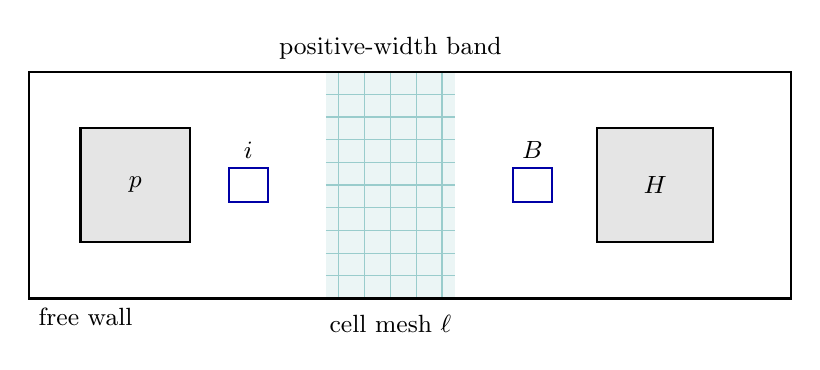
\begin{tikzpicture}[x=.82cm,y=.72cm,font=\small]
 \fill[teal!8] (4.6,0) rectangle (6.6,4);
 \draw[teal!40,step=.4] (4.6,0) grid (6.6,4);
 \draw[thick] (0,0) rectangle (11.8,4);
 \filldraw[fill=black!10,draw=black,thick] (.8,1) rectangle (2.5,3);
 \filldraw[fill=black!10,draw=black,thick] (8.8,1) rectangle (10.6,3);
 \draw[blue!65!black,thick] (3.1,1.7) rectangle (3.7,2.3);
 \draw[blue!65!black,thick] (7.5,1.7) rectangle (8.1,2.3);
 \node at (1.65,2) {$p$};
 \node at (9.7,2) {$H$};
 \node[above] at (5.6,4.05) {positive-width band};
 \node[above] at (3.4,2.3) {$i$};
 \node[above] at (7.8,2.3) {$B$};
 \node[below] at (5.6,-.12) {cell mesh $\ell$};
 \node[below right] at (0,0) {free wall};
\end{tikzpicture}
\caption{The band separates two positive-area pin regions.
The test boxes lie away from the band. Its cell mesh \(\ell\)
is refined while the physical band width stays fixed; the
band strength is increased only afterwards. Hard pins constrain
all primary height vertices in their regions.}
\label{fig:band}
\end{figure}


\begin{proposition}[Vanishing reach]\label{prop:pins-reach}
Under the band law, the probability that an exploration
starting in a fixed positive-area region on one side of a separating
positive-width band reaches a fixed closed region on the
other side tends to zero in \eqref{eq:pins-limit-order}.
The assertion includes exploration from a filled exterior
or from a primary hard-pin region before imposing its pin.
\end{proposition}

\begin{proof}
Choose finite small-cell coverings \(i\) on the starting
side and \(B\) on the target side, away from the band and
with positive clearances. Enlarge overlapping cells slightly
so every crossing path meets both coverings after rounding;
see Figure~\ref{fig:band}.
Concretely, first choose two separator strips, clipped to
the free component, with a fixed clearance \(\eta>0\) from
the band and the filled starting and target regions.
Then cover them by cells of radius \(\delta\ll\eta\).
A reaching path contains, in a fixed-factor enlargement
of the touched cell, a segment spanning \(c\delta\).
The path-Poincare constant on this rescaled patch depends
only on the fixed finite face and corner geometry, not on
\(\delta\); at a wall use the adjacent face-connected
rectangular pieces of that same component.
The primary path bound gives a uniform upper bound \(C_0\)
for the centered remaining average in a reached cell.
A logarithmic trial supported in a fixed ball away from
the band gives continuum prior variance at least
\(c\,a\log(1/\delta)-C\) for a cell of radius \(\delta\).
Cut the trial off at a radius \(\rho<\eta/4\) fixed before
\(\delta\). It pays no band mass. At a free wall or corner
restrict it to the component; this is an admissible Neumann
energy function. Its cell average is bounded below by
\(c\log(\rho/\delta)-C\), and its energy is at most
\(C\log(\rho/\delta)+C\), uniformly over the bounded cell
shapes. Thus shrinking the cells increases the prior lower
bound without increasing the path-anchoring constant.
Choose the covering cells so small that the prior variance
exceeds \(C_0+2c_0\), for some \(c_0>0\), uniformly in
\(\lambda\). At each fixed \(\lambda\), band convergence
gives the strict gap \(c_0\) on fine meshes.

For exterior exploration write \(h_B=e_B+u_B\), exposed
plus unexposed. The centered posterior is obtained by
zero-pinning visited vertices and increasing cable
precision. Thus its variance for \(u_B\) is at most
the full prior variance \(v_B\), and at most \(v_B-c_0\)
on a visit to \(B\). Restoring the tilt changes the
averaged second moment and cross term by \(o(1)\), by
the good- and bad-tilt estimates above. The identity
\(\E_Wh_B^2=v_B\) therefore gives
\(c_0\Prob_W(B\text{ reached})\le\E_We_B^2+o(1)\).
All contributing clusters are macroscopic, with a
threshold fixed by the separation from the starting set.
Sign resampling, with that same signless selection, yields
\begin{equation}
 c_0\Prob_W(B\text{ reached})
 \le\E_W\sum_{C\text{ meeting the starting set}}M_C(B)^2+o(1).
 \label{eq:pins-exterior-deficit}
\end{equation}

For the second deficit, bias the prior by \(|h_x|\),
where \(x\in B\), and expose only its cluster.
The pre-exposure second moment at \(i\) is at least
\(v_i\) by \eqref{eq:pins-size-bias}. The bias is measurable
at completed exploration, so cancels from the conditional
complement law. Its centered remaining variance is at
most \(v_i\), and at most \(v_i-c_0\) when the cluster
visits \(i\). Multiply the total second-moment comparison
by \(\E|h_x|\) and the primary averaging weight of \(x\),
then sum over \(x\in B\). This produces precisely the
weight \(M_C(B)\), not a count of microscopic clusters.
Only clusters reaching the band or \(i\) cause a
nonzero tilt or exposed term; the separating gaps make
all of them macroscopic. The estimates preceding the
proposition give
\begin{equation}
 c_0\E_W\sum_{C:C\cap i\ne\varnothing}M_C(B)
 \le\E_W\sum_C M_C(B)M_C(i)^2+o(1).
 \label{eq:pins-biased-deficit}
\end{equation}
Points with \(\E|h_x|=0\) contribute zero.

As \(\lambda\to\infty\), the inverse forms
\(T_\lambda^{-1}\) decrease to the inverse with every
energy function zero on \(K\). Weak energy compactness
and recovery by such functions prove this statement
directly. The hard band separates the sides, so its
cross covariance is zero. Equation~\eqref{eq:pins-cross}
therefore makes
\(\E\sum_CM_C(B)M_C(i)\) vanish in the prescribed order.
Truncate first at \(\max_CM_C(i)\le M\); on this event
the right side of \eqref{eq:pins-biased-deficit} is at
most \(M\) times that cross sum. Its remaining tail
vanishes uniformly as \(M\to\infty\), since
\[
             \sum_CM_C(B)M_C(i)^2\le\sqrt{Q_B}\,Q_i
\]
and Lemma~\ref{lem:pins-resampling} supplies arbitrarily
high moments uniform toward large \(\lambda\).
Consequently the first-mass sum on the left of
\eqref{eq:pins-biased-deficit} vanishes.
Every starting-set cluster meeting \(B\) visits one
of the finitely many cells \(i\). Truncate
\(\max_CM_C(B)\) in \eqref{eq:pins-exterior-deficit}
and use these first-mass bounds; its tail is controlled
by the moments of \(Q_B\). This proves vanishing reach.

All exploration calculations were on finite subdivided
Gaussian graphs. Their primary bounds are uniform in
large \(N\), or are passed first at a fixed primary
graph. Thus no continuum-time cable realization of the
limiting Bessel law is needed.
\end{proof}

\subsection{Mixed limits and relative hard-pin comparison}

\begin{proof}[Proof of Theorem~\ref{thm:mixed-limits}]
On a component meeting \(p\), start with a smooth shift
\(g\) vanishing near the entire pin but allowed to meet
the free walls. Choose a separating band between \(p\)
and its support, with fixed gaps. The band may be a
union of strips clipped to the component. Use the
ordinary mixed-domain geometry from \Bcite{an:mixed-scaling};
Lemma~\ref{lem:pins-path} already verifies its reference
inequalities at faces and junctions.

For the weak Neumann Laplacian test of \(g\), the band
variance is \(a\mathcal E_U(g)\).
Explore from every primary vertex of \(p\).
On success, the exposed test is zero and the centered
posterior has at least the desired primary pin, possibly
further zero pins, tighter chains, and restricted band
precision. Its variance is therefore at most that under
the desired massless hard-\(p\) law.
The tilt errors vanish as above. On failure the actual
second moment is bounded by its fourth-moment root
times the square root of the failure probability.
Lemma~\ref{lem:pins-band-density} bounds that fourth
moment uniformly after the first two limits and toward
large \(\lambda\). Proposition~\ref{prop:pins-reach}
therefore gives
\[
 \liminf_{n\to\infty}\Var_p(h,A g_n)
                  \ge a\mathcal E_U(g).
\]
Run the argument on an arbitrary primary subsequence.
The free variance upper bound gives the opposite
limsup. The free logarithmic transform upper bound
and the centered-variance lower bound under real tilt
then give the matching Gaussian Laplace limit.

Weak free-face terms may first be approximated by
bounded density smears in primary reference cost,
preserving their gap from \(p\) and the band.
The real mixed inverse-form approximation and density
of smooth shifts vanishing near \(p\), from
\Bcite{an:forms}, extend the result to all asserted
tests. Lemma~\ref{lem:reference-cost} controls the
errors independently of subdivision. It supplies
uniform integrability for every fixed linear
exponential and polynomial insertion.

Unpinned components were handled before
Lemma~\ref{lem:pins-band-density}. Finally integrate
a fixed finite-rank quadratic penalty against these
massless limits. On pinned components the preceding
moment bounds suffice. On unpinned components sum
translations and use the independent uniform
fractional mean, with the confining penalty controlling
the constants exactly as in the band-density proof.
This proves the theorem, including its limit order
and its statements for rounded geometry sequences.
\end{proof}

We now prove convergence of the interaction in
\eqref{eq:pins-definitions}; this is where a relative,
rather than absolute, estimate is essential.
Write \(U\) for the original finite box-average
penalty and \(W\) for a separating band penalty.
Let \(Z_{M,Q}\) be the partition sum with penalty
\(M\) and primary hard pin \(Q\). Cancellation gives
\begin{align}
 D_U-D_W
 &=\log\frac{Z_{U,H\cup p}}{Z_{W,H\cup p}}
   +\log\frac{Z_{U,\varnothing}}{Z_{W,\varnothing}}
   -\log\frac{Z_{U,H}}{Z_{W,H}}
   -\log\frac{Z_{U,p}}{Z_{W,p}}.
 \label{eq:pins-four-ratios}
\end{align}
Each ratio changes only a fixed finite-rank confining
penalty on one fixed massless pinned or unpinned
domain. Its common normalization cancels, so
Theorem~\ref{thm:mixed-limits} gives its Gaussian
limit at each fixed band partition and strength.
The real Gaussian determinant theorem
\Bcite{an:gaussian-localization} identifies the
corresponding interaction difference.

Under the unpinned band law, explore all clusters
meeting \(p\). On the event \(\mathcal S\) that
\(H\) is untouched, the centered posterior is
obtained from the band law conditioned on \(h_p=0\)
by further primary or internal zero pins and
increased precision. Its probability of \(h_H=0\)
is at least \(\mu_W(h_H=0\mid h_p=0)\).
For \(\epsilon\le\delta\le1\), the actual tilted
posterior therefore satisfies
\[
 \mu_W(h_H=0\mid\mathcal F)
 \ge e^{-C\delta^2}\mu_W(h_H=0\mid h_p=0).
\]
Averaging gives the relative estimate
\begin{equation}
 e^{-D_W}\ge e^{-C\delta^2}
                 \Prob_W(\mathcal S\cap\{\epsilon\le\delta\}).
 \label{eq:pins-relative-pin}
\end{equation}
It remains valid however small the two pin
probabilities are. By precision monotonicity
\(D_W\ge0\). First the tilt vanishes at fixed
\(\lambda\), then reach vanishes as \(\lambda\)
increases. Sending \(\delta\downarrow0\) proves
\(D_W\to0\) in \eqref{eq:pins-limit-order}.

The same vanishing holds for the real Gaussian
interaction \(D_W^{\mathrm g}\). One may use the
real-Gaussian proof of \Bcite{an:relative-pin-bound}:
replace pin probabilities by joint densities at
zero, use the same centered precision comparison,
and average small-box pin probabilities before
dividing by their volumes and applying Fatou.
The ordinary Gaussian localization theorem passes
the separated-pin determinants to the continuum.
Thus both band interactions vanish. Equation
\eqref{eq:pins-four-ratios} proves
\begin{equation}
                         D_n(H,p)\longrightarrow D^{\mathrm g}(H,p).
 \label{eq:pins-interaction-limit}
\end{equation}
No individual microscopic pin probability has been
assigned a positive continuum limit.

\subsection{Regression at typical pin data and restoration}

\begin{proof}[Proof of the remaining assertions of
Theorem~\ref{thm:pin-interaction}]
Let \(X_n\) be a fixed real smear,
\(m_n(b^p)=\E(X_n\mid h_p=b^p)\), and
\(v_{p,n}=\Var(X_n\mid h_p=0)\).
At prescribed primary data, the subdivided law is an
affine Gaussian lattice law with the same quadratic
part as at zero data. Lemma~\ref{lem:comparisons},
including an additional real tilt, and then its
fixed-graph limit give
\begin{equation}
       \Var(X_n\mid h_p=b^p;\text{ tilt }tX_n)\ge v_{p,n}.
 \label{eq:pins-conditional-variance}
\end{equation}

Choose the first \(J\) smooth density probes on \(p\),
and let \(L_n^{(J)}\) be their linear combination
with the limiting Gaussian regression coefficients.
Remove redundant directions or invert on their
Gram-matrix range. Conditional variance decomposition
gives the exact bound
\begin{align}
 \E|m_n-L_n^{(J)}|^2
 &=\E|X_n-L_n^{(J)}|^2
                   -\E\Var(X_n\mid h_p)\notag\\
 &\le \E|X_n-L_n^{(J)}|^2-v_{p,n}.
 \label{eq:pins-regression}
\end{align}
Theorem~\ref{thm:mixed-limits} identifies both limiting
variances. As \(J\to\infty\), totality of the pin
probes makes the right side tend to zero: in the
Gaussian energy space it is the squared difference
between the full pin projection and the \(J\)-probe
projection of the representer of \(X\).
Thus the conditional mean is approximated in \(L^2\)
by the finite Gaussian linear predictions.

Integrating \eqref{eq:pins-conditional-variance}
twice in \(t\) gives
\[
 Y_n:=\E(e^{X_n}\mid h_p)
             \ge\exp\{m_n+v_{p,n}/2\}.
\]
Both sides have limiting expectation \(e^{v/2}\),
where \(v\) is the full limiting variance.
For the right side, use \eqref{eq:pins-regression}
and uniform exponential integrability:
\(\E e^{q m_n}\le\E e^{qX_n}\) by Jensen for
every fixed real \(q\).
Their nonnegative difference tends to zero in
\(L^1\), proving the conditional Laplace assertion.
Apply the same argument to a countable dense set
of linear combinations of any fixed test list.
Subsequence extraction and conditional exponential
moment bounds give tightness and identify all
conditional finite-dimensional weak limits.
This also proves conditional convergence of fixed
smooth quadratic penalties.

For the pin ratio, precision comparison at prescribed
\(b^p\) shows that every normalized conditional
positive-penalty ratio is at most one and decreases
when the penalty is increased. Letting a full
coordinate pin on \(H\) tend to infinity yields
\(0<r_{H,n}\le1\). Its definition gives exactly
\(\E r_{H,n}=e^{-D_n}\).

Let \(Q_J\) be increasing finite smooth quadratic
penalties exhausting the pin on \(H\), and put
\[
 R_{J,n}(b^p)=
 \frac{\E(Q_J\mid h_p=b^p)}{\E(Q_J\mid h_p=0)}.
\]
Then \(r_{H,n}\le R_{J,n}\le1\).
For fixed \(J\), the conditional weak convergence
and the centered hard-\(p\) limit identify \(R_{J,n}\)
with its Gaussian counterpart. Moreover,
\begin{equation}
       \E(R_{J,n}-r_{H,n})=\E R_{J,n}-e^{-D_n}.
 \label{eq:pins-probe-gap}
\end{equation}
The interaction limit \eqref{eq:pins-interaction-limit}
and the finite-probe determinant approximation in
\Bcite{an:gaussian-localization} make the right side
tend to zero as \(J\to\infty\) after \(n\to\infty\).

More explicitly, let \(s_j\) be the singular values
of the cross projection between the Gaussian pin
spaces of \(p\) and \(H\). Positive separation gives
\(\sup_js_j<1\) and \(\sum_js_j^2<\infty\).
In canonical standard Gaussian pin coordinates
\(\xi_j\),
\[
 r_H^{\mathrm g}
 =\exp\left\{-\frac12\sum_j
           \frac{s_j^2}{1-s_j^2}\xi_j^2\right\}>0
 \quad\hbox{almost surely},\qquad
 \E r_H^{\mathrm g}=\prod_j\sqrt{1-s_j^2}=e^{-D^{\mathrm g}}.
\]
Finite probes exhaust these convergent expressions.
Markov's inequality in \eqref{eq:pins-probe-gap}
therefore proves the asserted finite-observation
approximation of the full ratio. In particular
\begin{equation}
 \lim_{\eta\downarrow0}\limsup_{n\to\infty}
                  \mu_n(r_{H,n}\le\eta)=0.
 \label{eq:pins-away-zero}
\end{equation}

Finally a fixed finite linear tilt has uniformly
bounded \(L^q\) density for every fixed finite \(q\):
its denominator is at least one, and the mixed
Laplace bounds control its numerator's moments.
Holder transfers the preceding convergence statements
to the tilted law. Here \(r_{H,n}\), \(D_n\), and the
conditional functions being sampled keep their centered
definitions; in particular we do not claim
\(\E_{\mu_{n,L}}r_{H,n}=e^{-D_n}\).
If a conditional transform under the tilted baseline is
needed, use
\[
 \E_{\mu_{n,L}}(e^X\mid h_p)
   =\frac{\E_{\mu_n}(e^{X+L}\mid h_p)}
          {\E_{\mu_n}(e^L\mid h_p)}.
\]
The denominator has a strictly positive Gaussian limit,
so the established joint conditional convergence applies.
This completes the theorem.
\end{proof}

\begin{lemma}[Restoration and two-way transfer]
\label{lem:restoration}
Let \(\mu_n\) be a cut centered high law and let
\(\nu_n\) restore bonds or positive forms supported
inside a core \(H\), separated from the guard \(p\).
Include both primary endpoints of every restored
bond, and the support of every restored form, in
the hard core pin. If \(Q_\Delta\) is the positive
restoration factor and
\[
 r_\Delta(b^p)=
 \frac{\E_{\mu_n}(Q_\Delta\mid h_p=b^p)}
      {\E_{\mu_n}(Q_\Delta\mid h_p=0)},
\]
then
\begin{equation}
 r_{H,n}\le r_\Delta\le1,\qquad
 \frac{\dd\nu_{n,p}}{\dd\mu_{n,p}}
   =\frac{r_\Delta}{\E_{\mu_n}r_\Delta},\qquad
 r_{H,n}\le\frac{\dd\nu_{n,p}}{\dd\mu_{n,p}}
                  \le e^{D_n(H,p)}.
 \label{eq:pins-restoration}
\end{equation}
Events concerning random guard data whose probabilities
tend to zero transfer in both directions between
the two topologies. This typical-data transfer also
holds when either law is sampled with a fixed finite
linear tilt. The displayed identities and inequalities
remain statements about the centered laws and their
centered-defined ratios.
\end{lemma}

\begin{proof}
For each restored edge \(e=(x,y)\), enlarge the cut
law by an independent normalized chain of increments
\(\xi_{e,1},\ldots,\xi_{e,N}\in2\pi\Z\) in height units, and put
\(J_e=\sum_k\xi_{e,k}\). Restoring the edge imposes
\(J_e=h_y-h_x\). Conditional on primary heights, its
factor is the chain-convolution probability
\(p_{b,N}((h_y-h_x)/(2\pi))\), tending to the Bessel
weight. Thus the primary factor need not itself be
quadratic. On the expanded lattice, matching is the
limit of the positive quadratic penalties
\(\exp[-t(J_e-h_y+h_x)^2/2]\).

Write \(Z_{b^p}\) and \(Z_0\) for the expanded cut
sums at the two guard data, and use a superscript
\(\Delta\) for restored matching and any further
restored positive forms. The guard fibers are affine
and centered copies of the same expanded lattice, and
\[
 r_\Delta(b^p)=
       \frac{Z_{b^p}^{\Delta}/Z_{b^p}}
            {Z_0^{\Delta}/Z_0}.
\]
Precision comparison gives \(r_\Delta\le1\);
adding the full primary \(H\)-pin can only decrease
this ratio. With both endpoints pinned, every new
chain matches \(J_e=0\). Its integrated factor is
the scalar \(p_{b,N}(0)>0\), independent of guard
data. Hence
\(Z_{b^p}^{\Delta+H}=\kappa_N Z_{b^p}^{H}\)
and \(Z_0^{\Delta+H}=\kappa_N Z_0^{H}\), with the
same \(\kappa_N\). The resulting normalized ratio is
exactly \(r_{H,n}\), proving its lower bound.
All independent-chain normalizers were identical in
these sums, and both they and \(\kappa_N\) cancel.
Internal chain variables therefore need not be pinned.
Take matching penalties to infinity and then the
fixed-primary-graph subdivision limit.

Bayes' formula gives the middle identity in
\eqref{eq:pins-restoration}. Its denominator lies
in \([e^{-D_n},1]\), proving the last two bounds.
The interaction has a finite limit, so the upper
density bound transfers \(\mu_{n,p}(A_n)\to0\)
to \(\nu_{n,p}(A_n)\to0\). Conversely, for \(\eta>0\),
\[
 \mu_{n,p}(A_n)
 \le\mu_{n,p}(r_{H,n}\le\eta)
                       +\eta^{-1}\nu_{n,p}(A_n).
\]
Use \eqref{eq:pins-away-zero}, sending \(\eta\downarrow0\)
after the lattice limit. Fixed linear tilts transfer
by Holder and the bounds for both positive and
negative fixed exponential moments. All these
statements concern the finite-observation sense at
typical data specified above.
\end{proof}

\section{Magnetic sectors and the spin lower bound}
\label{sec:magnetic}

Throughout this section, fix \(b>0\) with \(a=a(b)>0\).
We prove the converse to Proposition~\ref{prop:spin-upper}.

\begin{proposition}[Magnetic lower bound]\label{prop:spin-lower}
For the prescribed free-box correlation,
\[
 \liminf_{n\to\infty}\frac{\log C_b(n)}{\log n}
       \ge -\frac{2\pi}{a}.
\]
In particular, \(m(b)=0\).
\end{proposition}

Convergence of ordinary height observations does not by itself compare
partition functions in different winding sectors. We make that comparison
by adding confining observations on each of finitely many scales. Local
Gaussian limits then control guarded bond restorations, and an exact
finite expansion bounds the accumulated error. The high-law inputs are
Theorems~\ref{thm:mixed-limits} and~\ref{thm:pin-interaction} and
Lemma~\ref{lem:restoration}, already proved for the Skellam weights.
The real Gaussian localization estimates used below are the unchanged
ones in \Bcite{an:gaussian-localization}.

\subsection{A localized magnetic sector}

Use coordinates divided by \(n\), so the sources are \(0,e_1\).
Take the outer box sufficiently large that its boundary is well outside
\([-8,8]^2\) in these coordinates. There is a real multivalued function
\(v\), with periods \(2\pi,-2\pi\) at the two sources, which equals a
signed polar angle plus a smooth function near each source and has a
single-valued lift equal to zero outside \([-2,2]^2\). Indeed, the
difference of the two angles has zero period on an outer annulus;
multiply its lift there by a cutoff. Choose bounded-value branches,
with bounded integer jumps. Whenever a local chart is changed, apply
the same integer gauge to the lattice height and to \(v\).

Fix a large microscopic length \(m_*\). Choose \(q\) so that
\[
                 m_*\le 2^{-q}n\le 2m_*,
\]
and remove the dual height vertices in two open squares of half-side
\(2^{-q}\) about the sources, rounding their faces to lattice divisions.
The new inner walls are free. The prescribed connection still has the
two indicated periods in this punctured graph. Below, all observations
are outside the holes and are contained in charts missing the sources.

Let \(B\) be a collection of box averages, to be specified shortly.
Add the observation factor
\begin{equation}\label{eq:magnetic-mass}
 \exp\left\{-\frac12\norm{Bh-Bv}^2\right\}
\end{equation}
in the shifted sector and use target zero in the centered sector.
Equivalently, average the single-valued deviation in each chart.
The two targets and their connection can be chosen zero on a common
outer terminal region. Lemma~\ref{lem:comparisons} shows that adding
\eqref{eq:magnetic-mass} decreases the shifted-to-centered ratio:
in enlarged affine coordinates the new coordinates are \(Bh-Bv\),
versus \(Bh\) on the parallel centered lattice, and we are adding a
positive quadratic form. No integer-valued assumption on \(v\) is used.

Here is the geometry, including the uniformity needed later. First
choose a sufficiently large dyadic integer \(M\), and then a large
dyadic integer \(R\). There is a face-connected tessellation by regular
tiles and one unprocessed exterior object with the following properties.
\begin{enumerate}[label=(\roman*),leftmargin=*]
\item Away from outer termination, tile size is comparable to distance
to the nearer source divided by \(M\), with distance capped at a fixed
constant away from the sources. Each tile contains mass cells whose
side lengths are comparable to its size divided by \(R\).
\item Patches of every fixed tile-radius used below have a bounded
number of tiles, local charts missing the sources, and comparable
mass-cell sizes. Their pre-pin components, including after local bond
deletions, have the mixed geometry of Theorem~\ref{thm:mixed-limits}.
Guards and cores are unions of tiles; their intervening collars have
width comparable to \(R\) in mass-cell units. Mass cells do not cross
a guard or a tile cut.
\item There are at most \(C_M(1+\log n)\) processed tiles and uniformly
bounded face-graph degrees. On each fixed-radius patch, a target lift
has bounded magnitude and bounded sampled gradient energy, uniformly
in \(R,n\). Its vector of mass-cell averages has norm at most a fixed
polynomial in \(R\).
\item The exterior object starts beyond the support of the target,
contains the remaining graph up to the outer height pin, and is never
processed. An ordinary continuation of the local tessellation and
of the mass cells is retained through a wide collar of its inner
boundary. Local patches use this continuation and stay far from the
outer pin. For dependency counting only, tiles attached to the
exterior may be joined through one terminal node of degree bounded
in terms of \(M\); local distances never use this shortcut.
\end{enumerate}

To construct the tessellation, divide the sup-norm neighborhood of
radius \(1/4\) of each source into square rings with successive radii
in ratio two, down to its hole. Subdivide a ring into squares of side
its inner radius divided by \(M\); use a matching uniform grid in the
remaining bounded region. At subdivision junctions insert small
trimmed square tiles, with side a fixed fraction of the shortest
incident side. Clip at the holes when necessary. Thus point contacts
do not join components, and incident sectors which must be joined
have a face, rather than an opposite-only junction. This is the
geometry of \Bcite{an:geometry}. Subdivide all tiles and trimmed
parts into rectangular mass cells of the stated size, with compatible
face subdivisions. Rounded coordinates retain the same adjacencies
when \(m_*\) is large enough.

Choose the fixed patch, guard, skip, and enlargement radii first, and
take \(M\) larger than all of them. After rescaling by the local ring
radius, the patches and their possible local deletions range over
finitely many shapes, up to bounded lattice rounding. Here is why
this covers every integer \(n\), not just dyadic separations.
In primary lattice units the logical ring radii are \(r_j=n2^{-j}\),
stopped with \(m_*\le r_q<2m_*\). Round each shared logical face
once to a dual-lattice division, and reuse it on both sides.
Its displacement is \(O(1)\). A fixed-radius patch spans only
boundedly many neighboring ring scales, so its ideal normalized
shape and deletion pattern belong to finite lists. Its mesh
and face-rounding errors in mass-cell units are at most
\[
                         \frac{C_M R}{r_j}
                                  \le \frac{C_M R}{m_*}.
\]
For large \(m_*\), all widths, incidences, and collars are preserved.

The targets also range over compact smooth families. Near a
source \(z_0\), after scaling by \(\rho_j=r_j/n\), a local lift
has the form \(\pm\arg z+g(z_0+\rho_jz)\), with \(g\) smooth
and \(0<\rho_j\le1/4\). Adjoining \(\rho=0\) closes this
family in the required smooth norms; finitely many angle
charts suffice. The outer patches have fixed smooth families,
and bounded integer chart changes add finitely many choices.
Sampled cell averages converge uniformly on these compact sets.
If a common refinement threshold failed at fixed \(M,R\), a
sequence of failing patches with mesh tending to zero would
have a subsequence with one ideal shape and deletion pattern
and a convergent target. The admissibly rounded high-law and
real Gaussian limits on that subsequence give a contradiction.
Thus one fixed \(m_*(R)\) makes every local estimate below
uniform over all rings, all sufficiently large integer \(n\),
and all sufficiently distant outer boundaries. Guards can be
enlarged by whole tile layers, also at an inner free wall.

\begin{figure}[tbp]
\centering
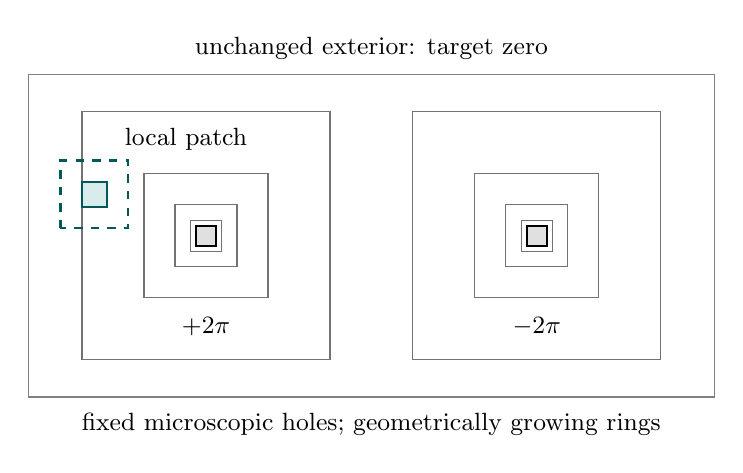
\begin{tikzpicture}[x=1.05cm,y=1.05cm,font=\small]
 \draw[black!50] (-4.15,-1.95) rectangle (4.15,1.95);
 \foreach \x in {-2,2} {
  \foreach \r in {1.5,.75,.375,.1875}
   {\draw[black!55] (\x-\r,-\r) rectangle (\x+\r,\r);}
  \fill[black!12] (\x-.12,-.12) rectangle (\x+.12,.12);
  \draw[thick] (\x-.12,-.12) rectangle (\x+.12,.12);
 }
 \filldraw[fill=teal!15,draw=teal!70!black,thick]
  (-3.5,.35) rectangle (-3.2,.65);
 \draw[teal!70!black,dashed,thick]
  (-3.76,.09) rectangle (-2.94,.91);
 \node[above right] at (-3.1,.91) {local patch};
 \node[fill=white,inner sep=1pt] at (-2,-1.1) {$+2\pi$};
 \node[fill=white,inner sep=1pt] at (2,-1.1) {$-2\pi$};
 \node[above] at (0,2.02) {unchanged exterior: target zero};
 \node[below] at (0,-2.03)
  {fixed microscopic holes; geometrically growing rings};
\end{tikzpicture}
\caption{Schematic geometry for the winding-sector comparison.
Each square ring is partitioned into tiles much smaller than its
distance to the source; only one tile and its enlarged patch are
shown. The construction trims tile junctions and uses collars
with full interfaces. The number of processed tiles is
\(O_M(1+\log n)\), while the unprocessed exterior is kept intact.}
\label{fig:annuli}
\end{figure}


Let \(Z^s,Z^0\) denote the punctured, observation-weighted partition
functions in the shifted and centered sectors. In the same finite
graph let \(Z_{\mathrm g}^s,Z_{\mathrm g}^0\) be the real Gaussian
integrals with gradient precision \(A/a\), the same observations,
outer zero wall, and periods. A free component has a confining
observation, so its constant is integrated rather than fixed.
In comparisons of the two models, a Gaussian pin probability
means the corresponding density at the prescribed coordinates,
or equivalently the common shrinking-neighborhood ratio.
Pin interactions and their determinant formulas are therefore
meaningful although individual Gaussian pin events have
probability zero.

\begin{proposition}[Many-scale sector comparison]
\label{prop:sector-comparison}
For the preceding geometry there are numbers \(\eta_R\to0\) such that,
for each sufficiently large fixed \(R\), one can choose a fixed
\(m_*\) for which
\begin{equation}\label{eq:magnetic-sector-comparison}
 \left|\log\frac{Z^s}{Z^0}
       -\log\frac{Z_{\mathrm g}^s}{Z_{\mathrm g}^0}\right|
       \le C_M(1+\log n)\eta_R.
\end{equation}
For these fixed choices, heights on the two inner rims, in the
bounded cut coordinates just specified, are uniformly tight in
\(n\) and in the outer volume. This is absolute tightness, without
subtracting an additive constant.
\end{proposition}

\subsection{An exact isolation expansion}

Fix an order of the processed tiles. An ordinary step deletes all
still-present bonds from its tile to other tiles, including the
exterior object. Around its core choose a free patch of fixed tile
radius, containing a separating guard and collars wider than any
later support enlargement. In the current local topology, let
\(U_o,U_c\) be the patch before and after this proposed deletion.
Both admit pure-gauge lifts. Replace the bond factor by the scalar
\begin{equation}\label{eq:magnetic-proxy}
 D_i^s=
 \frac{Z_{U_o}^0}{Z_{U_c}^0}
 \frac{Z_{\mathrm g,U_o}^s/Z_{\mathrm g,U_o}^0}
      {Z_{\mathrm g,U_c}^s/Z_{\mathrm g,U_c}^0}
\end{equation}
times the cut factor, plus their difference. In the centered
calculation omit the second fraction, obtaining \(D_i^0\).
For the real Gaussian expansion use its own centered constants
in the same formula.

Selecting the difference marks this step. After a mark, skip every
later step within a fixed number of tile layers, larger than all
patches and guard-testing boxes. Thus marks are separated, their
guard interiors are left untouched, and a subsequently considered
proxy cannot depend on which of the two positive terms is selected
inside a previous difference. This is a finite, exact expansion.
All deviations from the unmarked sequence are supported in bounded
halos of marks. At its end every surviving cross-tile bond, other
than a bond wholly within the exterior, lies in such a halo or
joins it to the exterior.

Normalize each sector by its no-mark term: the product of its
successive proxies and the final isolated tile partition functions,
including the unchanged exterior. For a specified set \(I\) of
\(j\) marks, write \(w(I)\) for its contribution divided by this
normalization.

\begin{lemma}[Pattern gain]\label{lem:magnetic-pattern}
For either model and either sector, after increasing \(m_*\) at
fixed sufficiently large \(R\),
\begin{equation}\label{eq:magnetic-pattern}
                         |w(I)|\le e^{-cRj}.
\end{equation}
Here and below \(c>0\) may decrease, and all fixed constants may
depend on \(b,a,M\), but not on \(n\) or the outer volume.
\end{lemma}

\begin{proof}
We separate the centered normalization, the random guards, and the
local gain.

\paragraph{Conditional differences.}
Prescribe all primary heights \(u_i\) on the guards of the marks.
Let \(K_o,K_c\) be the two positive partition kernels inside one
guard, in the corresponding marked step. Set
\[
 \delta_i(u_i)=
 \frac{|K_o-D_i^sK_c|}{K_o+D_i^sK_c}\le1,
\]
and use \(D_i^0\) in the centered sector. Guard and exterior factors
cancel from this expression. Conditional integration of the product
of differences, followed by the triangle inequality, gives a sum
of at most \(2^j\) positive topologies. In each one the integrand
has the additional factor \(\prod_i\delta_i\). We have not assumed
independence of the random guard data.

\paragraph{Centered normalization.}
For a positive topology \(G\), including its ordinary proxy factors,
its contribution divided by the no-mark term is at most
\begin{equation}\label{eq:magnetic-accounting}
 e^{Cj}\frac{Z_G^s}{Z_G^0}\,
                  \E_{G,s}\prod_i\delta_i.
\end{equation}
Only affected components are included in this display; untouched
final tile factors have been canceled.

Here is the accounting behind \eqref{eq:magnetic-accounting}.
A centered restoration supported in a core lies between its
free-patch value and its value with a separating guard pinned to
zero, whether the actual exterior is absent or present.
Lemma~\ref{lem:comparisons} gives the direction. For a chain
representation, retain the independent chain increments and
restore endpoint matching; all scalar chain normalizers are the
same in these comparisons. A full primary pin on a region \(H\)
containing the restored endpoints makes the restoration a fixed
scalar. Therefore its free-to-guarded multiplicative gap is at
most
\[
 \frac{\Prob(h_p=0\mid h_H=0)}{\Prob(h_p=0)}
                         =e^{D(H,p)}.
\]
Theorems~\ref{thm:pin-interaction} and
\Bcite{an:gaussian-localization} bound this uniformly, and in fact
make its logarithm exponentially small in \(R\) after sufficient
microscopic refinement. Indeed, gradient energy plus cell-average
mass is uniformly coercive in mass-cell units, the clearance is
of order \(R\), and local cell volumes are polynomial in \(R\).
The same cell-cutoff and Hilbert--Schmidt estimates apply to the
bounded rectangular shapes here, including at free walls.

Only \(O_M(j)\) such normalization comparisons are charged.
Take a union containing sufficiently enlarged halos of all marks,
with a further collar beyond every skip and dependence radius.
Telescope separately the actual centered partition functions along
the positive branch and along the no-mark branch in this union.
Include the whole exterior object and its neighboring collar if
surviving bonds or changes can meet it. Count every event in the
union, including one clipped at its artificial boundary. At a
clipped event use the proxy clipped in the same manner on both
paths. Before every boundary event, the two histories agree
on its entire proxy patch: the collar contains every affected
or skipped step and exceeds the proxy's dependence radius.
Thus the scalar change from an original proxy to its clipped
version is identical on both paths and cancels. There are
\(O_M(j)\) events; the exterior itself
has none. Final integrals and proxies outside the affected region
also cancel, while the initial centered integrals on the two paths
are identical. Each remaining true-to-proxy ratio is bounded by
the preceding centered sandwich. Enlarging by whole tile layers
ensures that clipped comparisons still have separating guards
with unchanged clearance. Artificial point contacts add no bonds.
More explicitly, call this induced union \(U\), with free
artificial walls, and let \(\alpha\) be either deletion history.
For an actual deletion \(e\), put
\[
 T_e^\alpha=\frac{Z_{U,e\text{ before}}^0}
                  {Z_{U,e\text{ after}}^0},
 \qquad \widetilde D_e^\alpha
       =\text{its centered proxy clipped to }U.
\]
A skipped step or an open marked choice is not a deletion;
a cut marked choice is a deletion and carries its proxy.
The exact telescoping identity is
\begin{equation}\label{eq:magnetic-centered-telescope}
 Z_{U,\mathrm{final}\,\alpha}^0
       \prod_{e\in\alpha}\widetilde D_e^\alpha
   =Z_{U,\mathrm{initial}}^0
       \prod_{e\in\alpha}\frac{\widetilde D_e^\alpha}{T_e^\alpha}.
\end{equation}
The initial integral is common to both histories. In their
quotient, changing an original proxy to a clipped one cancels
at the artificial boundary, where the histories agree through
a collar wider than the proxy radius. Final components outside
\(U\) are identical and have no surviving bond to \(U\);
including an attached exterior object ensures this also for
terminal connections. Each product on the right has \(O_M(j)\)
factors, each bounded with its inverse by the centered
sandwich, also up to a new free wall. An exterior object has
no deletion events, and its whole inner collar has only
\(O_M(1)\) tiles. Thus its arbitrarily large microscopic
volume adds no charge. This proves \(e^{Cj}\) without an
error proportional to untouched tiles, as in
\Bcite{en:normalization}.

The shifted proxy factors agree off the same halos. Within them
each Gaussian shifted minimum energy is bounded by a fixed
constant: try the local target lift, whose gradient energy is
bounded and whose observation error is zero. Likewise, each
isolated regular tile has shifted-to-centered ratio bounded
below by a fixed positive constant after refinement.
Theorem~\ref{thm:mixed-limits}, including summation of constants
and the uniform fractional mean, gives convergence to its
Gaussian ratio; the same target trial bounds its Gaussian energy.
These constants are uniform for large \(R\) once the microscopic
mesh has been chosen. The exterior alone is unshifted.
These facts give the remaining shift accounting in
\eqref{eq:magnetic-accounting}, even when an affected connected
component has no global lift.

\paragraph{Cutting with prescribed guards.}
Cut disjoint larger boxes of tiles around the marks, well outside
their guards. For joint partition weights \(J_G(s,u)\), normalized
at centered shifts and zero prescribed guard data, affine
comparison gives
\begin{equation}\label{eq:magnetic-guard-cut}
 \frac{J_G(s,u)}{J_G(0,0)}
       \le
 \frac{J_{G^{\rm cut}}(s,u)}{J_{G^{\rm cut}}(0,0)}.
\end{equation}
This includes the connection, observation shifts, and prescribed
primary heights as affine coordinates. Restoring the cut bonds
is an increase of precision, so Lemma~\ref{lem:comparisons}
applies. This is the comparison of \Bcite{en:shifted-box}, now
using the established Skellam comparison.

To return from zero prescribed data to unprescribed data, the
remaining centered factor is a ratio of probabilities that all
these guards are zero. Impose them successively. For each guard
use a still larger separating patch, disjoint from the cuts and
the previously imposed guards. Its centered pin probability in
the full and clipped graphs lies between common open-patch and
outer-pinned values, whose ratio is bounded by a separated
hard-pin interaction. Their product costs at most \(e^{Cj}\).
Skip distances were chosen large enough to keep these boxes
disjoint.

We may enlarge the affected region in
\eqref{eq:magnetic-accounting} to include every otherwise
untouched isolated tile in these boxes; their shifted ratios
cost at most another \(e^{Cj}\). Include the exterior object
whenever it is met. Sum \eqref{eq:magnetic-guard-cut} over the
data, keeping the same \(\delta_i\), since cutting beyond a
guard does not change its interior kernel. The outside
shifted-to-centered factor is at most one. Inside, the cut
boxes are independent and their own shifted-to-centered
factors are also at most one. All twists within a box are now
ordinary bounded observation shifts after integer gauge changes.
It remains to prove, in either of its two positive topologies,
\begin{equation}\label{eq:magnetic-local-gain}
                     \E_{{\rm box},s}\delta_i\le e^{-cR}.
\end{equation}

\paragraph{The local gain at typical data.}
Write \(K_t(y,u)\), \(t=o,c\), in a common bounded lift,
where \(y=Bv\), and cancel factors depending only on the guard
or its exterior. Put
\[
 R(u)=\frac{K_o(0,u)}{K_c(0,u)},\qquad
 r_\Delta(u)=\frac{R(u)}{R(0)},\qquad
 F_t(y,u)=\log\E_{t,0}(e^{\ip{y}{Bh}}\mid h_p=u).
\]
The common observation constant \(e^{-\norm y^2/2}\)
cancels as well. If
\[
 P_{\mathrm g}(y)=
 \log\frac{Z_{\mathrm g,U_o}(y)/Z_{\mathrm g,U_o}(0)}
           {Z_{\mathrm g,U_c}(y)/Z_{\mathrm g,U_c}(0)},
\]
the exact decomposition is
\begin{equation}\label{eq:magnetic-kernel-decomposition}
 \log\frac{K_o(y,u)}{D_i^sK_c(y,u)}
   =\log\frac{R(0)}{D_i^0}+\log r_\Delta(u)
       +F_o(y,u)-F_c(y,u)-P_{\mathrm g}(y).
\end{equation}
The first term is \(O(e^{-cR})\) in the refinement limit
by the centered sandwich. The full-core pin ratio \(r_H\)
of the \emph{cut centered law} satisfies
\(\log r_H\le\log r_\Delta\le0\), with \(H\) containing
the restored bonds. No separate scaling limit for
\(r_\Delta\) is required: this sandwich and the bounded
discrepancy \(\delta_i\) suffice.

Theorems~\ref{thm:mixed-limits} and~\ref{thm:pin-interaction}
give joint convergence of \(r_H\) and the conditional Laplace
terms in the finite-observation sense, at this fixed geometry.
They apply under the centered or tilted laws of either
topology. One can first analyze conditioning in the whole cut
box: its interior kernel given the full guard agrees with that
in any completion with the same interior and guard. Transfer
between cut and restored typical data follows explicitly as
follows. For their centered guard laws \(\mu_p,\nu_p\),
Lemma~\ref{lem:restoration} gives
\[
 r_H\le \frac{\dd\nu_p}{\dd\mu_p}\le e^{D(H,p)}.
\]
Thus \(\mu_p(E)\to0\) implies \(\nu_p(E)\to0\), and
\[
 \mu_p(E)\le \mu_p(r_H\le\kappa)+\kappa^{-1}\nu_p(E).
\]
Strict positivity of the limiting Gaussian \(r_H\), followed
by \(\kappa\downarrow0\), gives the converse. Taking a common
finite list of probes therefore makes both conditional
Laplace approximations and the pin-ratio approximation joint
under either law. Uniform fixed-tilt exponential moments
transfer exceptional sets to either tilted law by H\"older.
Probe exhaustion is after refinement at this fixed geometry.
Nothing here asserts a limit uniform at arbitrary microscopic
guard values.

For completeness, the quantitative Gaussian calculation is as
follows. Let \(u_c\) be the cut harmonic prediction from the guard
in the centered massive energy, and let \(\chi\) equal one on
the core and vanish before the guard. With \(T\) denoting the
gradient-plus-observation energy and \(y=Bv\), Gaussian
localization gives
\begin{equation}\label{eq:magnetic-prediction}
 \E\norm{\chi u_c}_T^2
       \le {\rm poly}(R)e^{-cR}(1+\norm y^2).
\end{equation}
This is the localized-operator and Hilbert--Schmidt estimate in
\Bcite{an:gaussian-localization}, or \Bcite{en:prediction}.
Restoration decreases centered guard covariance, and the
deterministic prediction due to the tilt is bounded by the
same localized operator. The Gaussian full-core pin ratio
satisfies
\[
                  -2\log r_H^{\mathrm g}
                         \le \norm{\chi u_c}_T^2.
\]
Indeed, subtracting this cutoff prediction makes the
conditional mean zero on the core without changing its guard
values. Orthogonal projection onto the restored admissible
space also bounds the change of prediction between cut and
restored topologies by \(\norm{\chi u_c}_T\). This remains
valid when restoration matches two previously free traces:
vanishing on the core is an admissible correction.
Thus the linear-in-data part of the conditional Laplace
discrepancy is bounded by \(C\norm y\norm{\chi u_c}_T\).
In fact, for \(f=B^*y\), centered Gaussian conditional means
\(m_t\), and conditional covariances \(C_t^p\),
\[
 F_o(y,u)-F_c(y,u)
  =\ip{f}{m_o(u)-m_c(u)}
       +\frac12\ip{f}{(C_o^p-C_c^p)f}.
\]
Here \(u_c=m_c(u)\) is always the cut-law prediction,
evaluated under either topology's data, and
\(\norm{f}_{T^*}\le\norm y\).

The conditional quadratic discrepancy from the open-patch
comparison is at most
\[
                    {\rm poly}(R)e^{-cR}\norm y^2.
\]
One way to see all of its
locality requirements is to compare the changes of the
minimized observation-energy matrices under restoration,
with and without the zero guard pin. Each change decays
exponentially as an observation index recedes from the core,
by positivity of the added form and a localized trial cut
off near restored edges. Near the core, the guard pin's
own effect decays from the guard. Cross entries follow
by positive-form Cauchy--Schwarz. The same argument at
the patch boundary compares the open patch with the full
box. There are only polynomially many entries; guard-only
and exterior terms cancel from the kernel ratio.
Finite guard probes can be exhausted after these estimates.
This is the projection argument underlying \Bcite{en:good-box}.

Here \(\norm y\le{\rm poly}(R)\), so all these bounds have an
exponentially small right side after weakening \(c\).
Use
\[
 \left|\frac{x-1}{x+1}\right|
                       \le\min\{1,|\log x|\},\qquad x>0.
\]
Convergence in probability of the finite-observation
approximations, the bound \(\delta_i\le1\), and Gaussian
localization prove \eqref{eq:magnetic-local-gain}, with slack.
At fixed \(R\), increase \(m_*\) so it holds uniformly over
the finite geometries and compact target families. Applying
it in the disjoint boxes, absorbing the factors \(2^j e^{Cj}\),
proves \eqref{eq:magnetic-pattern}.
\end{proof}

\subsection{Factorization, logarithmic errors, and rim insertions}

The pattern bound alone must be supplemented by exact dependence
information. Enlarge each mark halo past all skip and proxy radii,
and join two potential marks if their enlarged halos meet or
if they can attach to the same exterior terminal node. This
defines a graph of bounded degree, independent of \(R,n,L\).
For disconnected groups of marks the normalized weights factor.
Indeed, a skip depends only on nearby earlier marks, a considered
proxy only on the current cuts in its patch, and an unmarked
deletion isolates its tile. All final non-product integrals lie
inside halos, possibly attached to the exterior. Distinct groups
have disjoint variables and no surviving bonds between them.
If the exterior could connect them, they were joined through its
terminal node. The signed sums over final positive topologies
therefore factor as well, with the original global order merely
restricted to each group. All untouched factors cancel exactly.
Violations of the skip rule have weight zero, a condition
checked separately in each component.

Consequently the normalized partition is a finite gas of
compatible connected mark sets, with activities bounded by
\(e^{-cRj}\) for size \(j\). We record explicitly the smallness
argument for signed activities. In a graph of bounded degree,
there are at most \(D^j\) connected sets of size \(j\) containing
a given site, and their closed neighborhoods have at most
\(D'j\) sites. Let \(\Xi(V)\) be the gas partition sum when marks
are allowed only in a set \(V\); ordinary unmarked steps are
still retained. Removing one allowed site \(x\) and summing
over the connected polymer containing it gives
\[
 \frac{\Xi(V)}{\Xi(V\setminus\{x\})}-1
  =\sum_{\substack{P\ni x\\P\subset V}}
       w(P)\,
       \frac{\Xi(V\setminus N[P])}
            {\Xi(V\setminus\{x\})}.
\]
Induct on \(|V|\). If smaller deletion ratios lie in
\([1-\eps_R,1+\eps_R]\), the absolute value of the right side
is at most
\[
       \sum_{j\ge1}D^j e^{-cRj}(1-\eps_R)^{-D'j}.
\]
For sufficiently large \(R\), this is at most
\(\eps_R=O(e^{-c'R})<1/2\), after adjusting constants.
The induction gives nonvanishing and positivity, also for all
restricted sums, and
\begin{equation}\label{eq:magnetic-gas-log}
                         |\log\Xi(V)|\le 2\eps_R|V|.
\end{equation}
Thus signed cancellations cannot invalidate the logarithmic
estimate.

The shifted-to-centered ratios of corresponding no-mark proxies
are identical in the lattice and Gaussian models, by
\eqref{eq:magnetic-proxy}. For final isolated tiles their ratios
have arbitrarily small logarithmic discrepancies after refinement,
by Theorem~\ref{thm:mixed-limits} and the uniform fractional mean
in Theorem~\ref{thm:coefficient-gap}. Their Gaussian energies are
uniformly bounded by trying the target; hence the limiting
ratios are bounded away from zero. The isolated exterior has
ratio one. Apply \eqref{eq:magnetic-gas-log} to the two sectors
of both models. Since there are at most \(C_M(1+\log n)\)
processed tiles, this proves
\eqref{eq:magnetic-sector-comparison}, choosing all local
refinement errors smaller than a prescribed quantity tending
to zero with \(R\).

We next prove the tightness assertion of
Proposition~\ref{prop:sector-comparison}. For a primary inner-rim
site \(x\), insert \(e^{h_x}\) or \(e^{-h_x}\) in its bounded
cut coordinates. The microscopic volume of every fixed-radius
patch near \(x\) is bounded in terms of \(m_*,R,M\), also for
the rim translated to the other source. Add one distinguished
item at its tile in the preceding expansion. Discard difference
gains in a fixed neighborhood of this item; if an insertion
lies in a marked kernel, first bound the absolute difference
by the sum of its positive terms.

Clip a separate box about the distinguished item, including
all necessary neighboring tiles, while retaining disjoint
comparison boxes for more distant marks. Only boundedly many
ordinary gains have been discarded. The prescribed-guard
cutting inequality remains valid with the fixed real linear
tilt \(\pm h_x\) in the numerator, by
Lemma~\ref{lem:comparisons}. This uses monotonicity of the
tilted ratio, not the bound one for it. In the distinguished
box the ratio with the insertion is bounded by a finite
constant: each component has confining average penalties,
there are boundedly many lattice sites, the edge sums have
all fixed exponential moments, and translation sums are
Gaussian-confined. This constant may depend arbitrarily on
the fixed \(m_*,R,M\).
The inserted functional remains literally \(\pm h_x\)
throughout this comparison, not an extension by a flow or a
harmonic prediction. After cutting it is supported entirely
in the distinguished box. No matching constraint remains
to its exterior, so every other factor is untilted and has
shifted-to-centered ratio at most one. A bounded change of
chart contributes only a bounded scalar. The rounded
distinguished graphs form a finite set at fixed \(m_*\),
and their target vectors form compact sets, making the
finite insertion constant uniform for all integer \(n\).

The previous centered accounting applies with the distinguished
halo included. Connected weights containing the distinguished
item are therefore bounded by
\[
                       C_{m_*,R,M}e^{-cRj},
\]
where \(j\) is the number of ordinary marks; the bounded
number of lost gains is absorbed in the constant. All other
components factor as before. More explicitly, let \(*\) be
the forced distinguished item and let \(\Xi\) be the gas
without the insertion. Group the inserted expansion by the
connected component containing \(*\). With \(P\subset V\)
its ordinary marks, the exact normalized expression is
\[
 \E_s e^{\pm h_x}
   =\sum_{\substack{P\subset V\\P\cup\{*\}\ \mathrm{connected}}}
       W_*(P)\,
       \frac{\Xi(V\setminus N[P\cup\{*\}])}{\Xi(V)}.
\]
The weights include the finitely many altered factors in
the distinguished halo. For \(j=|P|\), their absolute values
are at most \(C_{m_*,R,M}e^{-cRj}\), the number of connected
choices is at most \(D^{j+1}\), and the removed neighborhood
has at most \(D'(j+1)\) sites. The deletion bounds proving
\eqref{eq:magnetic-gas-log} therefore dominate this expression
by
\[
 C_{m_*,R,M}
   \sum_{j\ge0}D^{j+1}e^{-cRj}
                    (1-\eps_R)^{-D'(j+1)}<\infty.
\]
This bound is independent of \(|V|\); no extensive
log-partition bound is used when dividing the two sums.
Consequently,
\begin{equation}\label{eq:magnetic-rim-moment}
       \E_s e^{h_x}+\E_s e^{-h_x}\le C_{m_*,R,M},
\end{equation}
uniformly in \(n,L\). There are boundedly many inner-rim sites
for fixed \(m_*\), so \eqref{eq:magnetic-rim-moment} proves
the asserted absolute tightness and completes the proof of
Proposition~\ref{prop:sector-comparison}.

\subsection{Filling the holes and the angular energy}

Return to the full dual partition of Lemma~\ref{lem:duality}.
First add the observation penalties, only outside the holes;
this lowers its shifted-to-centered ratio. Compare this
weighted full partition with its punctured version. With
normalized edge weights \(p_b\), the centered filling kernel
is bounded above by one: retain a spanning forest attaching
the finitely many removed vertices to their rim, sum the
forest increments using \(\sum_jp_b(j)=1\), and bound the
other edge factors by one. A fixed harmless normalization
convention would instead give a fixed upper bound.

By Proposition~\ref{prop:sector-comparison}, in the shifted
punctured law all adjacent rim values are bounded by a
fixed constant with uniformly positive probability.
Fill both holes with any fixed bounded configuration in
the cut coordinates. There are only finitely many required
integer differences, bounded in terms of the fixed choices,
including those on the continued offset path. All their
weights \(p_b(j)\) are strictly positive. Thus the numerator
filling factor is bounded below on this event by a positive
constant. We obtain
\begin{equation}\label{eq:magnetic-fill}
 \E_{\mu_{L,b}}\cos(\theta_0-\theta_{ne_1})
                         \ge c_{m_*,R,M,b}\frac{Z^s}{Z^0}
\end{equation}
uniformly for the large outer boxes under consideration.
The exterior dual face remains fixed at zero throughout,
which is the original free spin boundary condition; no
primal boundary spin has been fixed.

For the real Gaussian model, completing the square gives
the shifted-to-centered ratio as the exponential of minus
one half the minimum affine energy. Trying the sampled
target \(v\) makes the observation error zero and matches
the exterior pin. Therefore
\begin{equation}\label{eq:magnetic-energy}
 -\log\frac{Z_{\mathrm g}^s}{Z_{\mathrm g}^0}
       \le \frac1{2a}\bigl(4\pi\log n+O_{m_*}(1)\bigr).
\end{equation}
Indeed, near each source the angular energy is
\[
 \int_{m_*/n<|z|<c}|\nabla\arg z|^2\,\dd z
                        =2\pi\log n+O_{m_*}(1).
\]
Replacing the circular inner boundary by a square changes
only the bounded term. The other angle and the cutoff
corrections are smooth near that source; their cross terms
with its \(1/|z|\) gradient are integrable. All remaining
energies are bounded. On the lattice, derivative errors
of order \(r^{-2}\) at distance \(r\) give summable errors
in the squared-gradient sum. Thus the two singularities
give exactly \(4\pi\), with no extra factor from oriented
edge counting.

\begin{proof}[Proof of Proposition~\ref{prop:spin-lower}]
Choose \(M\), then arbitrarily large fixed \(R\), and then
sufficiently large fixed \(m_*\) as in
Proposition~\ref{prop:sector-comparison}. Combining
\eqref{eq:magnetic-sector-comparison},
\eqref{eq:magnetic-fill}, and \eqref{eq:magnetic-energy}
gives, uniformly in sufficiently distant outer boundaries,
\[
 \log \E_{\mu_{L,b}}\cos(\theta_0-\theta_{ne_1})
 \ge -\frac{2\pi}{a}\log n
       -C_M(1+\log n)\eta_R-O_{m_*,R,M,b}(1).
\]
For each fixed \(n\), first take the prescribed free-box
limit \(L\to\infty\). Divide by \(\log n\), and then
take the liminf as \(n\to\infty\). All hole and insertion
constants were fixed before this limit and disappear.
Finally let \(R\to\infty\), obtaining the claimed lower
exponent. Since \(0<C_b(n)\le1\), this polynomial lower
bound also implies \(m(b)=0\).
\end{proof}

\section{Openness above the marginal coefficient}\label{sec:openness}

We now exclude a supermarginal coefficient at the mass threshold.
The required assertion concerns the original Skellam height law:
\begin{proposition}\label{prop:openness}
If \(a(b)>8\pi\), there is an open interval \(I\) containing \(b\),
contained in \((0,\infty)\), such that \(a(\widetilde b)>0\) for
every \(\widetilde b\in I\).
\end{proposition}
We will not assume continuity of \(a\), nor differentiate it.  The
argument first adds a positive precision on \emph{block averages}.
This supplies a Gaussian large-field bound for the observed field,
while its scaling coefficient can be kept above \(8\pi\).
We prove entry into the small-activity maps at fixed reference, and
then use a torus variance diagnostic to return to the original model.

\subsection{A strengthened law and its local limits}

Fix \(b\) with \(a=a(b)>8\pi\).  Choose \(\delta>0\) sufficiently small
that
\begin{equation}\label{eq:op-reference}
 a'=(a^{-1}+\delta)^{-1}>8\pi,\qquad \alpha=\sqrt{a'}.
\end{equation}
Both \(\delta\) and \(a'\) remain fixed when the physical parameter
\(\widetilde b\) varies.  For a dyadic \(s_0\), let \(B_{s_0}\) average
over disjoint square cells of side \(s_0\), and let \(A_{\rm cell}\)
be the unit-conductance nearest-neighbor Laplacian on these cells.
Add to the height energy the term
\begin{equation}\label{eq:op-added-precision}
 \frac{\delta}{2}\ip{B_{s_0}h}{A_{\rm cell}B_{s_0}h}.
\end{equation}
All grids are nested and have the common square-symmetry origins
used below.  Set \(s=ts_0\), where \(t\) is also dyadic, and observe
\begin{equation}\label{eq:op-observation}
 Y=B_sh+\eta,\qquad \eta\sim N(0,\Id),
\end{equation}
with independent observation noise.  On tori we work modulo global
height translation by \(2\pi\).  When local observations confine a
component constant, its translations are summed instead.

The comparison observation is \(B_s\alpha\psi+\eta\), where the
mean-free covariance of \(\psi\) is \(A^+\) and its constant is
uniform modulo \(2\pi/\alpha\).  In particular, this is the
\emph{ordinary nearest-neighbor} Gaussian reference; no averaged
precision is added to it.  On a cut graph \(G\), write its minimized
observation energy as
\begin{equation}\label{eq:op-observation-energy}
 E_G(y)=\inf_v\left\{a'^{-1}\ip{v}{A_Gv}
                         +\norm{B_sv-y}_2^2\right\},
\end{equation}
using free constants on the components.  Denote by \(Z_G(y;\widetilde b)\)
the corresponding Skellam partition sum with
\eqref{eq:op-added-precision} and observation penalty
\(\norm{B_sh-y}_2^2/2\).

The local domains are the mixed polygonal patches of
Theorem~\ref{thm:mixed-limits}, aligned with whole \(s\)-cells.
Whenever microscopic bonds between tiles are deleted, delete also
the bonds of \(A_{\rm cell}\) crossing that cut.  Thus a pre-pin
component has precisely its own subcells and face bonds.  A hard
core pin used to dominate a restoration includes all primary
vertices in every subcell supporting a restored averaged bond.
Such supports fit inside the fixed core collars.

\begin{lemma}[Strengthened local limits]\label{lem:op-local-limits}
Fix a bounded mixed geometry in observation-cell units, with
separated positive-area core and guard pins and observation masses
controlling each unpinned constant.  At the central parameter \(b\),
the strengthened laws have the Gaussian smear, conditional-smear,
and pin-interaction limits of Theorems~\ref{thm:mixed-limits}
and~\ref{thm:pin-interaction}, with coefficient \(a'\), in the
iterated limit
\[
             \lim_{t\to\infty}\lim_{s_0\to\infty}.
\]
The limits hold under each indicated pin set.  The quantities
\(D\) and \(r_H\) retain their centered-law definitions;
finite-probe convergence of these conditional quantities holds
also when their data are sampled under any fixed real observation
tilt.  This is convergence in probability under the corresponding
guard laws, not a redefinition of the centered pin ratios.
At fixed geometry the conclusions are uniform on compact sets of
observation data.
\end{lemma}

\begin{proof}
For fixed \(t\), the additional energy is a finite-rank quadratic
tilt of finitely many subcell averages.  Theorems~\ref{thm:mixed-limits}
and~\ref{thm:pin-interaction} give its limit on each fixed pin set.
Integration against the nonnegative quadratic weight is justified
by its boundedness and the confining observation masses; fixed
linear tilts are handled by the exponential moment bounds.
Free component constants are treated by the joint uniform-phase
limit before summing their confining translations.

The full pin interaction also transforms by finite-dimensional
quantities.  If \(W\) is the added quadratic weight, and subscripts
indicate centered conditioning on the designated pins, then
\begin{equation}\label{eq:op-tilted-interaction}
 D_W(H,p)-D(H,p)
 =\log\E_{H,p}W+\log\E W
       -\log\E_HW-\log\E_pW .
\end{equation}
Each expectation has a strictly positive Gaussian limit.  This
proves, at fixed \(t\), convergence to the pin interaction for the
tilted continuum Gaussian precision, not merely convergence of
unconditioned smears.

In observation-cell units, let \(P_t\) denote averages over squares
of side \(1/t\), and \(B\) averages over the unit observation cells.
The continuum form obtained in this first limit is
\begin{equation}\label{eq:op-continuum-form}
 T_t(f)=a^{-1}\int|\nabla f|^2
       +\delta\sum_{\langle i,j\rangle}
                  \bigl((P_tf)_i-(P_tf)_j\bigr)^2
       +\norm{Bf}_2^2 .
\end{equation}
It converges in inverse forms to
\begin{equation}\label{eq:op-limit-form}
                   T(f)=a'^{-1}\int|\nabla f|^2+\norm{Bf}_2^2,
\end{equation}
also with any of the specified zero-region pins.  Here is the
form argument, including its normalization.  If \(\zeta=1/t\),
the averaged-gradient term is a sum of
\(\zeta^2|D_\zeta P_tf|^2\).  Bounded \(T_t\)-energy gives weak
\(H^1\) and strong \(L^2\) compactness on each fixed component.
The averaged difference quotients converge weakly to the
directional derivatives on its interior, giving the lower bound
with coefficient \(\delta\).  Conversely, smooth functions give
the matching upper bound by Riemann sums.  The averaged-gradient
term is uniformly bounded by a constant times continuum gradient
energy, by the two-cell Poincare inequality.  Energy approximation
therefore extends recovery to all admissible functions, using
corner cutoffs and density with zero neighborhoods of the pins,
as in \Bcite{an:forms}.  No component is glued through a point.
This proves the claimed inverse-form convergence and, in
particular, convergence of all finite covariance and pinned
inverse matrices.

We also need convergence of the infinite-dimensional interaction
determinant.  Form convergence alone would not give it.  We verify
the uniform compactness used in \Bcite{an:gaussian-localization}
for the additional averaged term.
For an energy-harmonic function off a pin or source, test its
equation against \(\chi^2f\), where \(\chi\) is a smooth cutoff
in a separating margin.  On a subcell replace
\((P_t(\chi^2f))_i\) by \(\chi_i^2(P_tf)_i\).  The error satisfies
\begin{equation}\label{eq:op-cutoff-error}
 \left|(P_t(\chi^2f))_i-\chi_i^2(P_tf)_i\right|
 \leq C\bigl(t^{-1}|\chi_i|+t^{-2}\bigr)
                         (P_tf^2)_i^{1/2}.
\end{equation}
Pairing this error with each incident averaged bond and applying
Cauchy--Schwarz absorbs the term with \(|\chi_i|\) into a fixed
part of the positive weighted bond energy.  The remaining
\(t^{-2}\) terms cost local \(L^2\) mass: use
\[
 |(P_tf)_i-(P_tf)_j|
       \leq(P_tf^2)_i^{1/2}+(P_tf^2)_j^{1/2}
\]
and the bounded number of incident bonds.  The differences of
the cutoff values themselves are controlled by the discrete
product inequality.  All bounds are uniform for large \(t\).

The unit-cell observation term may cross an intermediate cutoff.
On the fixed geometry its forcing consists of finitely many
bounded cell-average coefficients.  Carry these coefficients
as finite-dimensional coordinates through the successive
restriction maps.  Their bounds follow from the original energy
bound.  The remaining terms are local on an enlarged margin for
large \(t\).  We consequently obtain the same nested
gradient-from-\(L^2\) estimates as for the form with unit-cell
mass alone, with this fixed finite-rank enlargement.

Two broken-domain \(H^1\)-to-\(L^2\) compact embeddings, each
with singular numbers \(O(j^{-1/2})\), separated by these
harmonic interior estimates, give a uniform \(O(j^{-1})\)
singular-value tail for the cross projections between the
separated pin regions.  A fixed finite-rank enlargement changes
only finitely many singular directions.  Bounded-energy
sequences harmonic off one pin have weak limits harmonic off
that pin for \(T\): test their equations against smooth
functions, whose averaged differences converge strongly.
For a weakly null sequence, compact \(L^2\) convergence and the
interior estimate give strongly vanishing energy near the
other pin; the observation averages vanish as well.

For completeness, identify all the varying energy spaces with
the same broken \(H^1\) space \(V\).  The forms \(T_t\) are
uniformly equivalent there, since the original gradient and
observation terms are a lower bound and the averaged-gradient
term has a uniform upper bound.  Let \(V_{0,H}\) be the fixed
subspace of functions zero on \(H\).  Its \(T_t\)-orthogonal
complement \(U_H^t\) is the source projection space.  If
\(\phi\) is a smooth density supported in \(H\), orthogonality
of \(v_t\in U_H^t\) to the \(T_t\)-Riesz representative of
\(\phi\) is exactly \(\int v_t\phi=0\), independently of \(t\).

Take \(T_t\)-unit vectors in \(U_H^t\) orthogonal to increasing
finite lists of these probes.  Every weak limit vanishes on
\(H\) and is \(T\)-harmonic off \(H\), by the smooth-test
passage above.  It lies both in \(V_{0,H}\) and its
\(T\)-orthogonal complement, so is zero.  The finite
observation forcing coordinates are the actual averages
\(Bv_t\); strong \(L^2\) convergence makes them zero too.
For a cutoff \(\chi_p\) equal to one near the opposite pin,
the local estimate gives \(T_t(\chi_pv_t)\to0\).
Moreover
\(\norm{P_p^tv_t}_{T_t}\leq\norm{\chi_pv_t}_{T_t}\),
since \(v_t-\chi_pv_t\) vanishes on \(p\).  This proves
uniform finite-probe approximation of the cross projection.
The same argument applies in reverse, and the finite-probe
Gram matrices converge by inverse-form convergence.
Combined with the uniform square-summable singular tails,
these facts give convergence of the cross determinants.
The limiting cross projection has norm strictly smaller than
one, as in \Bcite{an:gaussian-localization}; operator convergence
preserves a norm gap.  In particular the logarithmic determinant
defining \(D(H,p)\) converges.

The conditional conclusions now follow by the regression and
minimal-Hessian argument used in Theorem~\ref{thm:pin-interaction},
with the covariance and determinant just obtained.  Conditional
Laplace transforms are first approximated using finitely many
smooth guard probes.  The full pin ratio follows by increasing
finite core penalties and using the centered identity
\(\E r_H=e^{-D(H,p)}\).
For use in both neighboring restoration topologies, take a
common finite probe list.  The bound
\(r_H\leq r_\Delta\leq1\) from Lemma~\ref{lem:restoration}, and
strict positivity of the Gaussian limiting \(r_H\), transfer
negligible exceptional sets in both directions.  Fixed real
tilts preserve convergence for these same centered-defined
quantities by the exponential moment bounds; the centered
expectation identity is not asserted under tilted sampling.

Every geometry and probe list is fixed before refinement.
Compact-data uniformity follows by taking convergent sequences
of observation vectors and using the same exponential
integrability.  Operationally, given an error tolerance one
first chooses a sufficiently large \(t\), then a sufficiently
large \(s_0\) depending on \(t\).  No single refinement threshold
uniform over all \(t\) is required.
\end{proof}

\subsection{A refinement-independent large-field reserve}

The bare quadratic energy of the subdivided Skellam law cannot
be used as a uniform site-level Gaussian tail.  The next bound
is the reason for adding \eqref{eq:op-added-precision}.

\begin{lemma}\label{lem:op-large-field}
For every cut topology used in the entry construction, there is
\(c_*>0\), depending only on \(\delta,a'\) and the fixed local
geometry conventions, such that
\begin{equation}\label{eq:op-large-field}
 \frac{Z_G(y;\widetilde b)}{Z_G(0;\widetilde b)}
                  \leq \exp\{-c_*E_G(y)/2\}.
\end{equation}
The same constant works for all sufficiently large dyadic
refinements and for \(\widetilde b\) in a neighborhood of \(b\).
\end{lemma}

\begin{proof}
On the subdivided quadratic lattice, complete the square in the
joint height and observation variables.  Centered theta
domination bounds the shifted sum by the centered sum times
the exponential of minus half its real minimum energy.
Discard the nonnegative microscopic chain energy in that
minimum, retaining the added average energy and
\(\norm{B_sh-y}_2^2\).  We show that this retained energy
dominates \(c_*E_G(y)\) for every real trial height.

Write \(u_i=(B_{s_0}h)_i\).  On the union of two adjacent
\(t\)-by-\(t\) subcell squares, the ordinary grid Poincare
inequality gives
\begin{equation}\label{eq:op-two-cell}
 |\overline u_{\rm left}-\overline u_{\rm right}|^2
 \leq \frac{2}{t^2}\sum_i|u_i-\overline u|^2
 \leq C\sum_{\langle i,j\rangle}(u_i-u_j)^2.
\end{equation}
The constant does not depend on \(t\).  Apply this to each
same-component observation face and sum with bounded overlap.
The observation residuals then show that
\begin{equation}\label{eq:op-face-control}
 \sum_{\langle x,x'\rangle\ {\rm in}\ G}(y_x-y_{x'})^2
 \leq C_\delta\left\{
       \delta\sum_{\langle i,j\rangle}(u_i-u_j)^2
                          +\norm{B_sh-y}_2^2\right\}.
\end{equation}
Only retained faces within a component occur.

Conversely, \(E_G(y)\) is at most a constant times the left
side of \eqref{eq:op-face-control}.  One explicit trial
interpolates the values \(y_x\) at scale \(s\), with central
plateaus and a piecewise affine subdivision joining cell
centers, face midpoints, and vertices.  At a midpoint or vertex
use the local average within each incident face-connected
sector.  Both its gradient energy and its observation error
are bounded by the nearby face-difference sum.  There is no
bond requirement between opposite-only sectors.  These local
estimates are uniform under the permitted cuts, and agree
under lattice refinement.  They prove the required comparison
of minima.

The constants do not use the microscopic chain precision or
the value of \(\widetilde b\).  Pass to the fixed-graph Skellam
limit using Lemma~\ref{lem:comparisons}.  If necessary decrease
\(c_*\) so that \(c_*\leq1\).  This gives
\eqref{eq:op-large-field} uniformly in the stated parameters.
\end{proof}

\subsection{Entry into the full analytic activity norm}

We use the nearest-neighbor Gaussian split and local subset
algebra of \Bcite{en:entry}.  The theorem there is stated for
quadratic discrete heights; it is \emph{not} being applied
directly to the present physical law.  We prove its needed
entry conclusion using Lemmas~\ref{lem:op-local-limits}
and~\ref{lem:op-large-field}, while retaining its
model-independent Gaussian estimates and finite expansion.

Fix admissible downstream parameters for \Bcite{wh:map} in
the gapped regime \(a'>8\pi\).  Write \(L\) for the block
factor, \(\mathfrak A\) for the activity weight, and \(h_0\)
for the analytic radius.  Choose with strict margins
\begin{equation}\label{eq:op-reserve}
 \max(0,1-c_*)<h_1<h_*<1/p_2,\qquad 1<p_1<p_2.
\end{equation}
The observation-energy regulator and norm are precisely those
of \Bcite{en:variational} and \Bcite{en:norm}, for this fixed
nearest-neighbor reference and these parameters.
For orientation, an activity \(K(X,\psi)\) is a local analytic
correction indexed by a finite set \(X\) of blocks; \(|X|\) is
its block count and \(\psi\) is the reference field.
The point norm \(|K(X)|_{u,X,\psi}\) includes the full sum of
field derivatives at analytic radius \(h_0\). At block side
\(u=mL^j\), the global norm is
\[
 \norm{K}_{u,\mathfrak A,V}
 =\sup_{X,\psi}\mathfrak A^{|X|}
   \frac{|K(X)|_{u,X,\psi}}
        {W_u^\kappa(X,\psi)e^{V_j(X,\psi)}}.
\]
The block supports and ordinary gradient regulator \(W_u^\kappa\)
are those of \Bcite{rg:geometry} and \Bcite{rg:regulator}.
The observation-energy regulator \(V_j\) is displayed in
\eqref{eq:op-regulator} below. Thus the entry estimate controls
all fields and analytic derivatives, not only bounded real data.

\begin{lemma}[Entry for the strengthened law]\label{lem:op-entry}
For every \(\epsilon>0\) there are fixed dyadic integers
\(q,R,t,s_0\), with \(P=R^5\), \(s=ts_0\), and \(m=qRs\),
and a real interval \(I\) about \(b\), such that the exact
relative observation density of the strengthened law, after
averaging the observation noise and reference modes below
scale \(m\), has plane and torus local subset activities
\(K_m\) satisfying
\begin{equation}\label{eq:op-entry-small}
       \norm{K_m(\widetilde b)}_{m,\mathfrak A,V}
                       \leq\epsilon\qquad(\widetilde b\in I).
\end{equation}
The norm includes the full analytic field-derivative sum.
The activities are real, even, square-covariant, invariant
under block-grid translations and common field translations
by \(2\pi/\alpha\).  The torus representation is exact for
compatible sides \(n\geq sP\), with exact plane copying on
unwrapped padded supports and the copying property under
subsequent local maps.
\end{lemma}

\begin{proof}
We give the entry estimates, especially the places where the
physical law differs from the quadratic source.
The choices are made in this order: the downstream norm and
regulator parameters and imaginary strip widths; \(q,R,P\);
a finite large-field threshold; \(t\); \(s_0\) depending on
\(t\); and finally the interval \(I\).

\paragraph{The reference split and exact expansion.}
For this observed law the exact density relative to its
Gaussian reference is, up to normalization,
\begin{equation}\label{eq:op-exact-density}
             Z_{\rm full}(y;\widetilde b)
                         \exp\{E_{\rm full}(y)/2\}.
\end{equation}
This is the observation identity \Bcite{en:exact-density}
with the new \(Z\).  Use the positive finite-range
nearest-neighbor covariance \(C_{<m}\) of
\Bcite{en:entry-covariance}, followed by its positive
finite-range shells.  These covariances, their ranges, and
the reference energies do not involve
\eqref{eq:op-added-precision}.

Use the covariant isolation of \Bcite{en:patches}: tiles of
diameter comparable to \(R\) observation cells, with trimmed
vertex tiles, finite colors of a fixed period \(q\), and
bounded-size proximity groups within each color.  The core,
open patch, and surrounding guard have fixed multiples of
\(R\) as their widths.  At an event, delete all remaining
bonds connecting its tiles to other tiles, counting each
bond once and deleting the corresponding averaged bonds.
If \(o,c\) are the current open patches before and after
deletion, use the replacement
\begin{equation}\label{eq:op-proxy}
 {\cal B}_i(y)=C_i\exp\{-(E_o(y)-E_c(y))/2\},\qquad
       C_i=\frac{Z_o(0;b)}{Z_c(0;b)}.
\end{equation}
The scalar is fixed at \(b\), while the Gaussian shape
always has reference \(a'\).  Replace the old weight by
this proxy times the cut weight plus their difference.
A selected difference marks the event and skips all later
events within a fixed sufficiently large halo.  This is an
exact finite expansion.  A later considered patch avoids
each earlier marked core and guard, so its proxy is
independent of the sign chosen inside that difference.

Divide by the product of the no-mark proxies and centered
isolated-tile normalizers.  Outside mark halos expand the
isolated error
\[
     \frac{Z_Q(y;\widetilde b)e^{E_Q(y)/2}}{Z_Q(0;b)}-1.
\]
The residual Gaussian quadratic difference between the full
energy and the no-mark energy is expanded into links, as
in \Bcite{en:link-matrix} and \Bcite{en:links}.  Gaussian
localization gives link weights \(Ce^{-c(R+d)}\) for length
\(d\), with their full displacement retained on tori.
All averaged-bond supports lie inside the required collars;
they change the physical positive topologies, not these
Gaussian link estimates.

\paragraph{Local normalization and cutting.}
For a marked core, its centered restoration ratio is
sandwiched between the open-patch ratio and the ratio with
its outer guard pinned to zero.  The logarithmic gap is
bounded by \(D(H,p)\), with \(H\) containing every restored
support.  This follows from Lemma~\ref{lem:restoration}
also for the additional positive averaged form.
Lemma~\ref{lem:op-local-limits} and Gaussian localization
make this gap exponentially small in \(R\), after the two
refinements at the fixed geometry.

Only \(O(j_1)\) centered comparisons are charged for
\(j_1\) marks.  Indeed telescope separately the positive
branch and no-mark branch on an enlarged union of their
halos.  The two paths agree at its artificial boundary,
so clipped proxies there cancel; final integrals and proxies
outside the affected union cancel as well.  All events
remaining inside the union number \(O(j_1)\).  This is the
finite double telescoping of \Bcite{en:normalization};
it applies unchanged to the present centered sandwich.
Finite-patch continuity preserves the bounded comparisons
near \(b\), with the constants \(C_i\) fixed as in
\eqref{eq:op-proxy}.  No error proportional to the
unaffected volume is introduced.

For a positive topology \(G\), the resulting bound has
the form
\begin{equation}\label{eq:op-pattern-before-cut}
 e^{Cj_1+Ce^{-cR}{\cal E}(y)}
 e^{E_G(y)/2}\frac{Z_G(y;\widetilde b)}{Z_G(0;\widetilde b)}
                  \E_{G,y}\prod_i\delta_i,
\end{equation}
where \({\cal E}\) is a face-difference cost in the padded
halo and, at prescribed primary guard data \(\gamma_i\),
\[
 \delta_i=
 \frac{|K_o(y,\gamma_i)-{\cal B}_i(y)K_c(y,\gamma_i)|}
      {K_o(y,\gamma_i)+{\cal B}_i(y)K_c(y,\gamma_i)}
                         \leq1.
\]
All factors exterior to a full guard cancel in this ratio.

Cut into \(P\)-boxes on an optimized translate of the
\(R\)-grid.  Averaging translates loses at most
\(C(R/P)j_1\) marks and costs at most
\(C(R/P){\cal E}(y)\) in Gaussian energy.  The joint
shifted-versus-centered comparison at prescribed guard
data is Lemma~\ref{lem:comparisons}, with the observations
embedded as height-plus-noise coordinates.  Its remaining
centered guard factors cost \(e^{Cj_1}\): impose the
guards sequentially and use open and zero-guard bounds
with separated outer collars.  Thus the cut comparison
has the same seam charge as \Bcite{en:seam-cost},
\begin{equation}\label{eq:op-seam}
                        e^{Cj_1+C(R/P){\cal E}(y)}.
\end{equation}

\paragraph{Bounded data and large data.}
We distinguish the graph used to classify observation data
from the positive topologies being compared.  Let \(D^0\)
be the observation-cell graph on the pattern's original padded
support \(D\), \emph{before any isolation deletion}.  Clip this
graph by the \(P\)-box grid and put
\begin{equation}\label{eq:op-original-face-cost}
 {\cal E}_{\rm box}(y)
 =\sum_{\substack{\langle x,x'\rangle\text{ in }D^0\\
                         x,x'\text{ in the box}}}
                                  (y_x-y_{x'})^2.
\end{equation}
In particular, a face remains in this cost when an isolation
step deletes its physical bonds.  Retain a deep mark only if
its complete open patch, restored supports, and guard lie in
the same clipped box; the other marks are among the boundary
losses already charged in \eqref{eq:op-seam}.  Thus every face
across which any retained restoration, Gaussian proxy, or
guard comparison tests a relative translation belongs to this
original graph.  Clipping adds no observation cell or exterior
field value to \(D\).

Fix the large-field threshold temporarily.  On each connected
component of this \emph{original} clipped graph translate all
heights, observations, and guard data together by one height
period, putting one observed value in \([-\pi,\pi]\).  Every
factor under comparison is invariant under this common
translation.  Bounded \({\cal E}_{\rm box}\) now gives a
compact set of observation values by following paths in the
finite original graph.  Independent translations of components
created by a later cut are not used: a restoration may join
those components and detect their relative translation.  At
fixed \(R,P\) there are finitely many geometries, positive
topologies, and mark choices.  Each Gaussian energy and each
physical partition function still uses its own actual positive
topology, not \(D^0\).

Decompose the logarithm of
\(K_o/({\cal B}_iK_c)\) into its centered zero-guard value,
the variation of its centered restoration with guard data,
and its two conditional observation Laplace terms minus
the Gaussian proxy change.  The first term is
\(O(e^{-cR})\) after refinement.  The second lies between
\(\log r_H\) and zero.  The conditional terms and \(r_H\)
converge by Lemma~\ref{lem:op-local-limits} under either
topology and its fixed observation tilt.

In the limiting Gaussian energy, let \(u_c\) be the cut
harmonic prediction from guard data and let \(\chi_H\)
equal one at the core and vanish before the guard.
The unchanged nearest-neighbor localization estimate
\Bcite{en:prediction} gives, for every \(r\geq2\),
\begin{equation}\label{eq:op-prediction}
 \left\|\norm{\chi_Hu_c}_T\right\|_{L^r}
 \leq C\sqrt r\,{\rm poly}(P)e^{-cR}
                         (1+\sqrt{{\cal E}_{\rm box}(y)}).
\end{equation}
The squared cutoff energy bounds \(-2\log r_H\).
Correcting a cut minimizer by this cutoff makes it
admissible for restoration without changing the guard;
orthogonal projection therefore bounds the linear
conditional-Laplace discrepancy by
\(C\norm{y}_2\norm{\chi_Hu_c}_T\).
The conditional quadratic discrepancy from the open-patch
proxy is bounded by \(Ce^{-cR}\norm{y}_2^2\), by the same
guarded localization.  These arguments use finite-energy
predictions and finite guard probes, not pointwise
continuum guard values.

Transfer these estimates using the conditional approximation
and \(r_H\leq r_\Delta\leq1\).  The Gaussian limiting
\(r_H\) is strictly positive, so exceptional sets are
negligible in both topologies, also after fixed tilts.
On such sets use \(\delta_i\leq1\).  Since
\(|(x-1)/(x+1)|\leq\min(1,|\log x|)\), bounded moments
of each \(\delta_i\) have the bounds from
\eqref{eq:op-prediction}.
Holder over the at most \({\rm poly}(P)\) deep marks,
and absorption of polynomial losses, give
\begin{equation}\label{eq:op-good-box}
 C\exp\{-cRj_{\rm deep}
                       +R^{-12}{\cal E}_{\rm box}(y)\}.
\end{equation}
For example, maximize
\((1+{\cal E})^{Cj}e^{-R^{-12}{\cal E}}\).
Since \(j\leq{\rm poly}(P)\), a factor
\([P^Cj^C(1+{\cal E})^C]^j\) is bounded by
\(e^{O(j\log R)+R^{-12}{\cal E}}\).
The \(O(j\log R)\) loss is absorbed by the exponential
rarity.  We use this smaller allowance so that the conservative
\(P^2\) coordinate count is negligible below.
Isolated selected-tile errors
can be made smaller than \(e^{-cR}\) by the same compact
Gaussian convergence.

We also need a separate estimate after a difference is expanded
into its two positive terms.  For every actual positive box
topology \(G\), Lemma~\ref{lem:op-local-limits} gives
\[
 e^{E_G(y)/2}\frac{Z_G(y;b)}{Z_G(0;b)}\longrightarrow1
\]
uniformly on the good-data compact set just described, after
the common period recentering.  The reference limit is precisely
the Gaussian of coefficient \(a'\), on that same topology.
There are only finitely many such topologies.  Choose the
refinements so that, on every good box,
\begin{equation}\label{eq:op-positive-good-box}
 e^{E_G(y)/2}\frac{Z_G(y;\widetilde b)}{Z_G(0;\widetilde b)}
       \leq 2\exp\{R^{-12}{\cal E}_{\rm box}(y)\}.
\end{equation}
At \(\widetilde b=b\) choose the stronger upper bound \(3/2\)
using that convergence; finite-patch continuity gives the bound \(2\)
after shrinking the eventual parameter interval.  For an
isolated-tile error expanded into its positive terms, the
constant Gaussian term satisfies the same bound.  Centered
normalizations between branches cost the already proved
\(e^{Cj_1}\).  Equation~\eqref{eq:op-positive-good-box}
therefore bounds positive branches without any discrepancy
factor \(\delta_i\); it is not obtained by removing
\(\delta_i\) from \eqref{eq:op-good-box}.  The displayed
allowance is retained to use the same quadratic-cost accounting
in both estimates.

On a bad box discard rarity and apply
Lemma~\ref{lem:op-large-field}.  Its centered-normalized
factor is at most
\[
 e^{E_G(y)/2}\frac{Z_G(y;\widetilde b)}{Z_G(0;\widetilde b)}
                     \leq e^{(1-c_*)E_G(y)/2}.
\]
This replaces the bare quadratic estimate
\Bcite{en:bad-box}.  It is the only large-field input
needed from the physical height law.

\paragraph{Gaussian averaging with reserve.}
Here is the energy accounting for the original-face costs.
For any real trial field \(v\) on the uncut padded domain,
two-cell Poincare and the observation residual give
\begin{equation}\label{eq:op-original-face-control}
 \sum_{\langle x,x'\rangle\text{ in }D^0}(y_x-y_{x'})^2
 \leq C\{a'^{-1}\ip{v}{A_Dv}+\norm{B_sv-y}_2^2\}.
\end{equation}
Indeed insert the two cell averages of \(v\) in each
difference.  The difference of averages is bounded by the
gradient energy on the two adjacent cells, as in
\eqref{eq:op-two-cell}; the two residuals are charged at
most four times.  All faces are internal to \(D^0\), so
these two-cell regions are present before minimization and
have bounded overlap, also at a clipped boundary.  Minimizing
over \(v\) proves the bound by \(CE_D(y)\).  This argument
does not ask a cut topology to control a deleted face.

For every positive branch of the expansion, restriction of
that same uncut trial field to the disjoint cut boxes bounds
the sum of their actual minimized energies \(E_G\) by
\(E_D\).  The bad-box physical contribution is consequently
at most \((1-c_*)E_D/2\).  All remaining data costs---the
\(R^{-12}{\cal E}_{\rm box}\) good-box allowance, seam
and halo costs, Gaussian links, and
\(\varepsilon_1{\cal E}_{\rm box}\) bad-box threshold
charges---use faces of \(D^0\).  Their summed coefficients
are at most
\(C(R^{-12}+R/P+e^{-cR}+\varepsilon_1)\) per face.
For halos this follows from their bounded multiplicity;
for links one sums their exponentially decaying displacement
weights.  The same bound applies to every restoration branch.
Choose \(R\) large and then \(\varepsilon_1>0\) small so
that \eqref{eq:op-original-face-control} makes their total
less than \([h_1-(1-c_*)]E_D/2\).  Thus the total positive
quadratic cost is at most \(h_1E_D/2\), with strict reserve
as required by \eqref{eq:op-reserve}.  The large-field
threshold is chosen only after this reserve is fixed.

The reference covariance contracts the observation
energy, exactly as in \Bcite{en:energy-contraction}.
At scale \(u=mL^j\), the regulator is
\begin{equation}\label{eq:op-regulator}
 V_j(X,\psi)=\frac12\sup_{\zeta,e}
 \left\{h_*E_{D_u(X)}\bigl(B_s\alpha(\psi+\zeta)+e\bigr)
       -p_1^{-1}\bigl(\norm{\zeta}_{<u}^2+\norm e_2^2\bigr)\right\}.
\end{equation}
Here the first norm is the Cameron norm of the reference
pieces below \(u\); singular covariances mean their
Gaussian Hilbert spaces.  The covariance contraction
and \(p_1h_*<1\) make this supremum finite.  Its
composition, localization, and terminal bounds are
\Bcite{en:regulator}; these involve only the unchanged
reference covariance and whole observation cells.

The determinant actually integrated is charged by its
localized quadratic costs, not by the larger dominating
form \(h_1E_D\).  Its trace is bounded by
\begin{equation}\label{eq:op-trace}
 C\,{\rm poly}(P)N_{\rm bad}
 +CR^{-12}P^2N_{\rm good}
 +C(R/P)R^2(j_1+j_2)
 +C\sum_\ell e^{-c(R+d_\ell)}{\rm poly}(d_\ell).
\end{equation}
Here \(N_{\rm good}\) counts occupied good boxes.
Broad bad-box terms, including their threshold charges,
have rank \(O(P^2)\).  The good-box allowance in
\eqref{eq:op-good-box} contributes at most
\(CR^{-12}P^2\) per occupied box, counting all present
cells of the clipped box.  Here \(P^2\) is only an upper
bound on their number; the actual quadratic cost remains
inside \(D\).  A halo intersects a bounded number of
\(P\)-boxes, so \(N_{\rm good}\leq C(j_1+j_2)\).
The remaining non-broad halo terms have coefficient
\(O(R/P)\) on \(O(R^2)\) observation cells, and links
retain their exponentially small path costs.
The added physical precision is contained inside \(Z_G\);
it is not a term of this reference Gaussian cost matrix.
Covariance contraction
gives a spectral margin below one, so logarithmic
determinant costs are bounded by a fixed multiple of
this trace.  No determinant counts subcells or
microscopic height variables.

Insert on a bad box the upper bound
\[
 1\leq\exp\{\varepsilon_1(
                    {\cal E}_{\rm box}(y)-U_{\rm big}^2)\},
\]
with sufficiently small fixed \(\varepsilon_1>0\).
Choose the finite \(U_{\rm big}\) to pay the polynomial
bad-box losses, the first term of \eqref{eq:op-trace},
and the lost item gains.  This choice precedes \(t,s_0\).
Since \(P=R^5\), both the full good-box allowance
\(R^{-12}P^2\) and the halo seam trace cost are
\(O(R^{-2})\) per item.  Gaussian completion with reserve consequently
gives, for an averaged pattern \(F_\pi\),
\begin{equation}\label{eq:op-real-pattern}
 |F_\pi(\psi)|
 \leq C^{j_1+j_2}e^{-cR(j_1+j_2)}
       \prod_\ell Ce^{-c(R+d_\ell)}
                     W_m^{\kappa_0}(X,\psi)e^{V_0(X,\psi)},
\end{equation}
where \(\kappa_0<\kappa\) leaves ordinary regulator
reserve.  A real translate by \(xf\), with \(f\) of
scaled point norm at most one, costs at most
\(e^{Cx^2|X|}\), with the final regulator still evaluated
at \(\psi\).  This uses \(h_1<h_*\) in the optimized
quadratic form and
\(\ip{f}{A_Df}\leq C|X|\).

\paragraph{Imaginary directions and analytic derivatives.}
The full analytic norm cannot be inferred from
bounded-real-data convergence alone.  On the extended
quadratic lattice, including
\eqref{eq:op-added-precision}, the theta parity identity
\Bcite{en:theta-parity} gives
\begin{equation}\label{eq:op-complex-comparison}
 \frac{|Z_G(y+iz;\widetilde b)|}{Z_G(y;\widetilde b)}
             \leq\frac{Z_G(iz;\widetilde b)}{Z_G(0;\widetilde b)}.
\end{equation}
It survives the fixed-graph Skellam limit.  The centered
imaginary ratio is its Gaussian prefactor times a
positive characteristic function; centered pinning
increases that characteristic factor.

Expand differences into positive topologies, temporarily
discarding their rarity, and apply
\eqref{eq:op-complex-comparison} to each whole integrated
topology.  Pin strips of width \(R/4\) along translated
\(P\)-box walls.  All walls and strip boundaries are
on observation-cell boundaries: \(R\) is dyadic,
\(R/4\) is integral, and the translates use the
\(R\)-grid.  Thus strips are unions of whole
observation cells and of their nested subcells;
no observation average is split.  Cutting through their interiors
disconnects also the averaged bonds, because all their
supporting subcells there are pinned.  On the resulting
bounded boxes, Lemma~\ref{lem:op-local-limits} gives the
Gaussian imaginary ratios uniformly on bounded
imaginary directions, with an arbitrarily small
multiplicative error after refinement.  Their limits
are strictly positive on each such compact set.

The additional Gaussian wall energy, averaged over wall
translates, is at most
\[
             C\norm z_\infty^2(R/P)
                         \#\{\hbox{active observation cells}\},
\]
by \Bcite{en:imaginary-wall}.  The other imaginary
Gaussian shapes cancel those of the proxies.  Real
parts are bounded on good boxes by the separate
positive-topology estimate \eqref{eq:op-positive-good-box},
and on bad boxes by Lemma~\ref{lem:op-large-field}.
Apply the preceding Gaussian completion to these bounds,
including the explicitly charged
\(CR^{-12}P^2N_{\rm good}\) term in
\eqref{eq:op-trace}; links retain their gains.
For fixed strip height \(H\) we obtain
\begin{align}\label{eq:op-rough-strip}
 |F_\pi(\psi+(x+iy)f)|
 &\leq
 \exp\{o(R)(j_1+j_2)+C_H(1+x^2)|X|\}
       \prod_\ell Ce^{-c(R+d_\ell)}
       W_m^\kappa(X,\psi)e^{V_0(X,\psi)},\nonumber\\[-2pt]
 &\hspace{65mm}|y|\leq H .
\end{align}
In particular, the wall charge per halo is
\(O(R^3/P)=O(R^{-2})\), not \(O(R^2)\).
Absolute Gaussian integration and analyticity follow
from \eqref{eq:op-large-field} with reserve and these
strip bounds.

Choose \(r_0>4eh_0\), then \(H>4r_0\), before \(R\).
Apply three-lines on the upper and lower strips to
\(F_\pi(\psi+zf)e^{-D_0z^2|X|}\), with \(D_0>C_H\).
The real boundary has \eqref{eq:op-real-pattern} and
the real-translation bound; the other boundary has
\eqref{eq:op-rough-strip}.  On \(|z|\leq r_0\) the
real-boundary harmonic weight is at least \(3/4\), so
the exponential item gains survive with a smaller
constant.  Removing the damping costs
\(e^{C|X|}\), absorbed because
\[
 |X|\leq C(j_1+j_2)+C\sum_\ell(1+d_\ell/R).
\]
Cauchy's estimate and real polarization bound the
order-\(r\) contribution to the analytic point norm
by the pattern bound times
\((h_0/r_0)^r r^r/r!\).  Its sum converges.  Thus
\eqref{eq:op-real-pattern}, with weaker constants,
holds in the full analytic point norm.

\paragraph{Uniformity and completion of entry.}
At fixed \(R,P\), choose a sufficiently large \(t\),
then a sufficiently large \(s_0\) depending on \(t\),
using Lemma~\ref{lem:op-local-limits} on the finitely
many bounded geometries, real-data compact sets, and
imaginary-direction compact sets just used.  All
estimates have strict slack.  Fixed-graph sums and
conditional bounded integrals are continuous in
\(\widetilde b\).  Indeed guard dimension is now
finite and fixed.  Although guard values range over
an unbounded lattice, \(\delta_i\leq1\), and the joint
laws and fixed tilts have uniform spanning-forest
exponential domination on the compact parameter and
observation sets.  Their positive normalizing sums
have positive compact lower bounds.  Dominated
convergence therefore applies to the integrated
absolute differences; no pointwise uniform estimate
at arbitrary guard data is needed.  Hence a
common real neighborhood of \(b\) preserves these
bounded-data estimates.  The global large-field
bound already has a uniform reserve.  The same
Gaussian averaging and interpolation therefore give
the full norm bound throughout this neighborhood;
no continuity assertion about the unknown \(a(\widetilde b)\)
has entered.

Finally use the connected pattern summation of
\Bcite{en:placement}.  A halo has bounded block
diameter and only polynomially many observation-cell
labels per block.  A link of length \(d\) covers
at most \(C(1+d/R)\) blocks.  The exponential item
and link gains pay all activity weights, coverings,
and rooted-tree sums, leaving \(Ce^{-cR}\) in the
norm.  Choose \(R\) large enough for
\eqref{eq:op-entry-small}.  Absolute estimates
justify every exchange with Gaussian integration.
Finite-range covariance factorization gives the
exact subset algebra, including its exclusions.
The covariant tile rules and aligned added form
preserve the stated symmetries.  The activity hypotheses
preceding \Bcite{wh:map} require block translations
and square symmetries, not unit-site translation
invariance of the physical interaction; the nested
grids have \(s_0\mid s\mid m\) and common square
centers.  Winding links keep
their full covers; every unwrapped padded support
therefore has exactly its plane activity.  This
proves the lemma.
\end{proof}

\subsection{Uniform gapped stability and a torus diagnostic}

We finish the proof of Proposition~\ref{prop:openness}.
Apply \Bcite{wh:map} with the cosine coordinate omitted,
which is permitted because \(a'>8\pi\).  The reference
kernel is fixed and nearest-neighbor; take its starting
scale sufficiently large.  The modified regulator is
allowed by \Bcite{en:regulator}.  All map hypotheses now
concern the reference and the small activities supplied
by Lemma~\ref{lem:op-entry}.

We record why the permitted smallness can be chosen
\emph{before} the large entry scale.  The Gaussian-curve
construction \Bcite{ep:gaussian-curves} gives exact
trajectories by initializing a small multiple \(d\)
of the block gradient energy and no lattice factor.
Their expansion has a linear gradient singleton and
an \(O(d^2)\) remainder.  These estimates are uniform
over sufficiently large starting scales: scaled block
gradient energy has a uniform point norm, and its
small exponential is absorbed by the same regulator
reserve.  Terminal Gaussian completion is also uniform,
because the tail covariance contracts the kinetic
energy and the terminal torus has a fixed number of
blocks.  On a fixed complex disk,
\((\Id-dC^{1/2}AC^{1/2})^{-1}\) is uniformly bounded,
and determinants cancel in the shifted ratios.
The map contraction and terminal gradient diagnostic
then prevent a first exit on that disk, exactly as
in the proof of \Bcite{ep:gaussian-curves}.  Its
analytic inverse disk is consequently uniform in
the starting scale as well as the RG step.  This
uniformity is a consequence of that proof and
\Bcite{en:regulator}, rather than an extra physical
assumption on the strengthened model.

Use the exact Gaussian parameter \(u\) for the
gradient coordinate and subtract the corresponding
Gaussian remainder, writing the transverse remainder
as \(B_{\rm rem}\).  The balanced linearization is
contracting transversely and the pure Gaussian curve
has no drift.  The analytic map estimates give
\begin{align}
 \norm{B_{{\rm rem},+}}
 &\leq[\theta+C(|u|+\norm{B_{\rm rem}})]
                                      \norm{B_{\rm rem}},\label{eq:op-gapped-B}\\
 |u_+-u|
 &\leq C(|u|+\norm{B_{\rm rem}})
                                      \norm{B_{\rm rem}}.\label{eq:op-gapped-u}
\end{align}
These are the fixed-reference inequalities
\Bcite{ep:gapped-B} and \Bcite{ep:gapped-u}.
Choose a small tube so that the first factor is at
most \(\theta'<1\).  Small enough entry data stay
in that tube, with
\(\norm{B_{{\rm rem},j}}\leq
(\theta')^j\norm{B_{{\rm rem},0}}\) and summable
gradient drift.  In particular all activities
remain as small as desired.  The separate torus
remainder obeys the same uniform small bound by
its contraction with quadratic forcing and the
exact copying of singleton coefficients in
\Bcite{wh:map}.

Choose a sufficiently large fixed dyadic \(D\) for
the causal neighborhoods of these maps and use
compatible tori of side
\begin{equation}\label{eq:op-stopping-tori}
                        n_j=DmL^j .
\end{equation}
Take \(j\) large enough that \(n_j\geq sP\), so
the exact entry is available.  At the stopping
scale there are \(D^2\) blocks.  Let \(f\) be a
nonzero mean-free first cosine on the unit torus,
and let \(f_n\) be its area-weighted observation-cell
samples.  Put
\[
                   g=\ip{f}{(-\Delta_{\T^2})^{-1}f}>0.
\]
The reference variance of \(\ip{Y}{f_n}\) tends
to \(a'g\).  Gaussian completion of a smooth real
source translates the exact relative density by
the reference covariance of that source.  The
Gaussian Laplace prefactor remains, while the
fixed terminal block count and regulator reserve
bound the differentiated logarithmic correction
by the small terminal activity norms.  This is
the gradient diagnostic
\Bcite{ep:gradient-diagnostic}.  It requires only
smallness here, not convergence of the gradient
coordinate to zero and not a derivative in
\(\widetilde b\).  By choosing the tube small,
for all sufficiently large \(j\),
\begin{equation}\label{eq:op-positive-torus}
 \Var_{\rm strengthened}\ip{Y}{f_{n_j}}
                                      \geq \tfrac12 a'g .
\end{equation}
The observation noise has variance
\(\sum_x f_{n_j}(x)^2=O((s/n_j)^2)\), which tends
to zero.  Removing the added positive precision
increases centered height variance by
Lemma~\ref{lem:comparisons}.  Hence the original
periodic Skellam height law satisfies
\begin{equation}\label{eq:op-original-torus}
 \liminf_{j\to\infty}
 \Var_{\widetilde b,{\rm tor}}
             \ip{h}{B_s^*f_{n_j}}>0
                    \qquad(\widetilde b\in I).
\end{equation}

If \(a(\widetilde b)=0\), the left side must instead
vanish.  To see this directly, first take a smooth
periodic gradient test.  Split the torus into
macroscopic rectangles, release the bonds between
them, and retain the internal gradient observations.
For a fixed macroscopic partition there are \(O(n)\)
seam edges and their coefficients are \(O(n^{-1})\),
so the discarded seams have reference cost \(O(n^{-1})\);
the free-cell variances converge to zero by
Theorem~\ref{thm:free-limits}.  The variance comparison
and Lemma~\ref{lem:reference-cost} give vanishing
variance for the original periodic test.  The
same conclusion holds for smooth mean-zero
density tests by using the periodic inverse
Laplacian and reference-energy approximation.
Finally, the observation-cell profile
\(B_s^*f_n\) approximates the corresponding
smooth density in reference cost as \(n\to\infty\),
with reference-cost error \(O((s/n)^2)\),
since \(s\) is fixed.  Equivalently one may use
the sampled periodic cosine shift and estimate
its cell-averaging error.  Thus its variance
also tends to zero, contradicting
\eqref{eq:op-original-torus}.

It follows that \(a(\widetilde b)>0\) throughout
the real neighborhood \(I\).  Shrinking \(I\)
inside \((0,\infty)\) proves
Proposition~\ref{prop:openness}.

\section{Identification of the critical exponent}
\label{sec:critical}

\begin{proof}[Proof of Theorem~\ref{thm:main}]
Apply Proposition~\ref{prop:spin-upper} at \(b=b_c\).
If \(a(b_c)=0\), it gives
\[
 \limsup_n\frac{\log C_{b_c}(n)}{\log n}=-\infty,
\]
whereas Proposition~\ref{prop:critical-lower} gives a liminf of at least
\(-1\). Hence \(a(b_c)>0\), and
Theorem~\ref{thm:coefficient-gap} implies
\[
                         a(b_c)\ge8\pi.
\]
Suppose the inequality were strict.
Proposition~\ref{prop:openness} would give \(a(\widetilde b)>0\)
for all \(\widetilde b\) in a neighborhood of \(b_c\).
Since \(b_c>0\), this neighborhood contains some
\(0<\widetilde b<b_c\).
Proposition~\ref{prop:spin-lower} then gives a polynomial lower
bound for \(C_{\widetilde b}(n)\), and therefore
\(m(\widetilde b)=0\): indeed \(C_{\widetilde b}(n)\le1\), and
its negative logarithm is \(O(\log n)\).
This contradicts \eqref{eq:critical-definition}. We have proved
\[
                              a(b_c)=8\pi.
\]
Propositions~\ref{prop:spin-upper} and~\ref{prop:spin-lower}
now give
\[
 -\frac14
 \le\liminf_n\frac{\log C_{b_c}(n)}{\log n}
 \le\limsup_n\frac{\log C_{b_c}(n)}{\log n}
 \le-\frac14.
\]
Both estimates use the free-box limit first and then all integer
separations, so they establish exactly the limit in the theorem.
The quantified bounds follow from the definition of this limit.
\end{proof}

The conclusion does not assert convergence of
\(n^{1/4}C_{b_c}(n)\). In particular, multiplicative logarithmic
corrections are compatible with the result.

The proof claims rest on the arguments and cited results presented here.
\begin{thebibliography}{99}
\raggedright

\bibitem{AHPS2022}
M.~Aizenman, M.~Harel, R.~Peled, and J.~Shapiro.
Depinning in integer-restricted Gaussian fields and BKT phases of
 two-component spin models.
\href{https://arxiv.org/abs/2110.09498v3}{arXiv:2110.09498v3},
May 27, 2022; first posted in 2021.

\bibitem{Berezinskii}
V.~L.~Berezinskii.
Destruction of long-range order in one-dimensional and
two-dimensional systems having a continuous symmetry group.
I.~Classical systems.
\emph{Soviet Physics JETP} \textbf{32}(3) (1971), 493--500.
Russian original: \emph{Zh. Eksp. Teor. Fiz.} \textbf{59}
(1970), 907--920.
\href{https://www.jetp.ras.ru/cgi-bin/dn/e_032_03_0493.pdf}
{English translation}.

\bibitem{DurandLammers2026}
T.~Durand and P.~Lammers.
The BKT transition and surface tension differentiability.
\href{https://arxiv.org/abs/2605.28473v1}{arXiv:2605.28473v1},
May 27, 2026.

\bibitem{FS}
J.~Fr\"ohlich and T.~Spencer.
The Kosterlitz--Thouless transition in two-dimensional Abelian
spin systems and the Coulomb gas.
\emph{Communications in Mathematical Physics}
\textbf{81}(4) (1981), 527--602.
\href{https://doi.org/10.1007/BF01208273}
{doi:10.1007/BF01208273}.

\bibitem{Ginibre1970}
J.~Ginibre.
General formulation of Griffiths' inequalities.
\emph{Communications in Mathematical Physics} \textbf{16}(4)
(1970), 310--328.
\href{https://doi.org/10.1007/BF01646537}{doi:10.1007/BF01646537}.

\bibitem{Kosterlitz1974}
J.~M.~Kosterlitz.
The critical properties of the two-dimensional XY model.
\emph{Journal of Physics C: Solid State Physics}
\textbf{7}(6) (1974), 1046--1060.
\href{https://doi.org/10.1088/0022-3719/7/6/005}
{doi:10.1088/0022-3719/7/6/005}.

\bibitem{BKT1973}
J.~M.~Kosterlitz and D.~J.~Thouless.
Ordering, metastability and phase transitions in two-dimensional systems.
\emph{Journal of Physics C: Solid State Physics}
\textbf{6}(7) (1973), 1181--1203.
\href{https://doi.org/10.1088/0022-3719/6/7/010}
{doi:10.1088/0022-3719/6/7/010}.

\bibitem{LammersBijecting2023}
P.~Lammers.
Bijecting the BKT transition.
\href{https://arxiv.org/abs/2301.06905v2}{arXiv:2301.06905v2},
April 18, 2023.

\bibitem{LammersDichotomy2026}
P.~Lammers.
A dichotomy theory for the height functions of the BKT transition.
\href{https://arxiv.org/abs/2211.14365v4}{arXiv:2211.14365v4},
July 25, 2026; first posted in 2022.

\bibitem{Lupu2016}
T.~Lupu.
From loop clusters and random interlacements to the free field.
\emph{The Annals of Probability} \textbf{44}(3)
(2016), 2117--2146.
\href{https://doi.org/10.1214/15-AOP1019}{doi:10.1214/15-AOP1019}.

\bibitem{McBryanSpencer1977}
O.~A.~McBryan and T.~Spencer.
On the decay of correlations in \(SO(n)\)-symmetric ferromagnets.
\emph{Communications in Mathematical Physics} \textbf{53}(3)
(1977), 299--302.
\href{https://doi.org/10.1007/BF01609854}{doi:10.1007/BF01609854}.

\bibitem{BKT}
OpenAI.
BKT universality for height and planar spin fields.
OpenAI Math Release preprint
\href{https://github.com/openai/math/blob/main/preprints/BKT-universality-for-height-and-planar-spin-fields-September-24-2026/paper.pdf}{OAI:BKT-universality-for-height-and-planar-spin-fields-September-24-2026},
2026.
All numbered companion citations refer to this paper.

\bibitem{RSD}
O.~Regev and N.~Stephens-Davidowitz.
An inequality for Gaussians on lattices.
\emph{SIAM Journal on Discrete Mathematics}
\textbf{31}(2) (2017), 749--757.
\href{https://doi.org/10.1137/15M1052226}
{doi:10.1137/15M1052226}.
\href{https://arxiv.org/abs/1502.04796v3}{arXiv:1502.04796v3}.

\bibitem{vEL}
D.~van Engelenburg and M.~Lis.
An elementary proof of phase transition in the planar XY model.
\emph{Communications in Mathematical Physics}
\textbf{399}(1) (2023), 85--104.
\href{https://doi.org/10.1007/s00220-022-04550-3}
{doi:10.1007/s00220-022-04550-3}.
\href{https://arxiv.org/abs/2110.09465v2}{arXiv:2110.09465v2}.
The multiplicative correlation inequality is cited from Lemma~19
of the appendix to this arXiv version; that appendix is absent
from the journal article.

\bibitem{vanEngelenburgLisDuality2025}
D.~van Engelenburg and M.~Lis.
On the duality between height functions and continuous spin models.
\emph{Probability and Mathematical Physics} \textbf{6}(4)
(2025), 1291--1325.
\href{https://doi.org/10.2140/pmp.2025.6.1291}{doi:10.2140/pmp.2025.6.1291}.

\end{thebibliography}

\end{document}
